\documentclass{article}
\usepackage[utf8]{inputenc}
\usepackage[hidelinks=true]{hyperref}
\usepackage{dirtree}
\usepackage{float}
\usepackage{minted}
\usepackage{graphicx}
\usepackage[a4paper]{geometry} % total={6in, 8in}
\usepackage[section]{placeins}

\usepackage[isbn=false, doi=false, eprint=false]{biblatex}
\addbibresource{data601.bib}

\usepackage{mathpazo, palatino}  %Check font in chapter style section too
\usepackage[LGR, T1]{fontenc}
\usepackage{bm}

% \renewcommand\thesection{\arabic{section}}
% \renewcommand\thesubsection{\thesection.\alph{subsection}}
% \renewcommand\thesubsubsection{\thesubsection.\roman{subsubsection}}

\newcommand{\ttt}[1]{{\texttt{#1}}}

\title{\textbf{Using Data Science Methods to
Investigate Philosophical Discourse in Early New Zealand Newspapers} \\ DATA601 Project Report}
\author{Joshua Black (46086757) \\ Word count: 10,664}

\begin{document}

\maketitle

\begin{abstract}
  Data science methods provide new opportunities for researchers in the humanities to explore
  large-scale text corpora. This report presents DATA601 summer project work
  with the UC Arts Digital Lab exploring philosophical discourse in
  New Zealand newspaper content up to 1900 using the
  recently released National Library Papers Past newspaper open data pilot
  dataset.

  The project has two parts.
  First, a corpus of texts is constructed for the
  investigation of philosophical discourse in early New Zealand newspapers.
  This is carried out using a `bootstrapping' method to generate increasingly
  targeted collections of articles. Second, the value of the resulting corpus is demonstrated by using it to explore two specific research questions. First, it is used to investigate the understandings of the relationship between religion and the natural sciences present in the corpus. Second, it is used
  to argue that a sizeable minority of articles in the corpus attempt to apply philosophical concepts to the New Zealand situation.
\end{abstract}

\tableofcontents

\section*{Introduction}

This project has two aims. First, to produce a corpus for the investigation of philosophical writing in early New Zealand newspapers.
Second, to illustrate the value of the resulting corpus by using it to
answer two specific research questions about such writing.

This project has been enabled by the release of the National Library Papers Past newspaper open data pilot \cite{ppnodp}. This is a large dataset of newspaper content running from 1839-1899.\footnote{
The dataset does not contain any Māori niupepa content.} While, the first newspaper content was made available in 2000 \cite{pp-about}, not many projects have attempted to use it as \emph{data}.\footnote{For instance, not many of the sample projects in the National Library's collection of \cite{ppnodp-projects} use Papers Past, and none of those which do use it as data to answer digital humanities research questions.}
The process of corpus construction carried out in this project reduces this dataset down from 7592619 articles to 31131 articles, which contain material interesting to the historian of philosophy. It is expected that the kind of methods and workflows developed in this project can be used profitably by other investigators to answer their own specific research questions about the Papers Past dataset.

Corpus construction was carried out using a `bootstrapping' approach with a combination of exploratory corpus analysis methods and supervised learning techniques. Beginning from simple keyword searches on the dataset, a series of articles of interest, and a variety of articles which were not of interest, were labelled and then used to train a Naive Bayes classifier. This classifier was then applied to the whole dataset. Further articles were then labelled using the corpus obtained from the classifier and then used to train a more effective Naive Bayes classifier.

Having constructed the corpus, two more specific research areas are considered. First, the attitudes to the relationship between religion and science present in the corpus. Second, the presence of specifically New Zealand content in the corpus.

This report is divided into four sections. The first discusses the humanities motivations of the project and sets out the three research questions which guide the project. The second section covers the corpus construction phase, discussing the methods used, issues with their implementation, and the nature of the resulting corpus. The third section demonstrates the use of the corpus developed in the previous section by using topic modelling, concordancing, and co-occurrence network analysis to investigate two specific questions about philosophical discourse in early New Zealand newspapers. The fourth section presents a critical discussion of the project, highlighting its successes and shortcomings. An appendix contains some large tables of results which are referred to in the report.

\section{Organisation, Motivation and Research Questions}

\subsection{UC Arts Digital Lab}

This project was carried out within the UC Arts Digital Lab at the University of Canterbury, under the supervision of Geoffrey Ford (Political Science) and Benjamin Adams (Computer Science).

The UC Arts Digital Lab works in the interdisciplinary area of `digital humanities'. Digital humanities is the application of computational and data science techniques to handle research and material traditionally studied by humanities disciplines. This includes digital archiving and computational analysis of, e.g., texts, audio and video, to gain insight into human culture.

This project falls within digital humanities by using data from a digital archiving project, the National Library's digitisation of New Zealand newspapers, and by applying data science techniques to extract relevant material and analyse it. That is, it combines data science methods with the traditional humanities aim of generating insights about cultural products.

Digital humanities is in its early stages of development in New Zealand. It is hoped that this project will demonstrate some of the potential of the data sources and resources available in New Zealand for novel work in this area.

\subsection{Project Motivations}\label{s:project-motivations}

This project picks out and investigates philosophical discourse in early New Zealand newspapers. This section provides some working definitions of important terms, sets out some of the motivations for carrying out the project and presents three research questions which will direct the project as a whole.

For the purpose of this project, `philosophical discourse' will be discourse which concerns ultimate values or ultimate reality. It will also have a special connection with argumentation. For instance, in many political speeches the concept of 'liberty' is used. Reflection on, and argument for, a particular idea of what liberty means would count as philosophical discourse (in this case, philosophical discourse about ultimate values) (e.g. \cite{bruce-liberty}). Similarly, reflection on whether there is a God is discourse about what is ultimately real (e.g. \cite{oxford-god}). Philosophy, in this sense, can be carried out both as an academic subject in the universities by specialists in the field and as a public activity by `non-professionals'.

Often the history of philosophy is a history of \textit{academic} philosophy. This leaves not much to say about philosophy in New Zealand until the well into twentieth century. Davies notes that, before this time, ‘many of those who had longstanding [academic] chairs published next to nothing’ and that the Australasian (and especially New Zealand) philosophical community was small and not well connected \cite[24]{davies-2014}. It has also been noted that academic philosophy in New Zealand has tended to simply follow international trends, with a `New Zealand philosophy' as something to be hoped for in the future \cite[ix--x]{oddie-1992}. These limitations in the usual focus on academic philosophy in the New Zealand context encourage the attempt to look for philosophical discourse elsewhere. Early New Zealand newspapers are a plausible place for us to look.
There is even reason to think that the relative lack of intellectual journals in New Zealand at the time, when compared with the UK, means that New Zealand newspaper contained more intellectual content than would be otherwise expected \cite[37]{crane-2013} \cite{ballantyne-2012}. Ballantyne has, in the context of a discussion of colonial Otago, described the newspaper as `the fundamental infrastructure for intellectual life' at the time \cite[57]{ballantyne-2012}.\footnote{
Another indication of significant connections between newspapers and philosophy in Australasia is Barzillai Quaife. One of the first newspapers in New Zealand, \textit{The New Zealand Advertiser and Bay of Islands Gazette}, was produced by Quaife, a Congregationalist minister who went on to be the first professional philosophy teacher in Australia and to publish \textit{The Intellectual Sciences}, a book which has a claim to being the first philosophical monograph produced in Australasia \cite[16--17]{davies-2014}. This example is singular, but further encourages the idea that early intellectual life, and philosophy in particular, may be traceable through early New Zealand newspapers.}

The turn to newspaper writing to investigate philosophical discourse in early New Zealand is enabled by the availability of digital humanities and data science methods. The availability of more than seven million articles in digital form allows for the application of text processing methods to highlight content which might otherwise be missed or to allow `reading' of more articles than it would be feasible for a single researcher to explore. This is, to use Moretti's phrase, `distant reading', as opposed to `close reading' \cite[47--49]{moretti}.\footnote{For a note of warning about treating this material as simply a `store of information' see \cite[59-60]{ballantyne-2012}.}

\subsection{Research Questions}

The project is structured by three research questions, as follows:
\begin{enumerate}
  \item Can supervised learning methods be used to produce a useful corpus for investigation of philosophical discourse in Early New Zealand Newspapers from the National Library Papers Past Newspaper Open Data Pilot dataset?
  \item Can the resulting data set be used to provide insight into how the relationship between religious belief and developments in the natural sciences was understood in early New Zealand?
  \item Can topic modelling and co-occurrence analysis on the resulting corpus reveal that philosophical writing in New Zealand newspapers incorporates concerns which are specific to New Zealand?
\end{enumerate}

The first question concerns corpus construction. The criteria for success in corpus building are not straightforwardly quantifiable and require qualitative judgement. In particular, a sustained qualitative investigation of the false positives and negatives produced by candidate classifiers will be required.
We will also examine the resulting corpus to determine if the articles it contains are relevant to the historian of philosophy and test for the presence of articles identified as of interest by previous studies but not used in the process of corpus construction.\footnote{Note that the test using articles from previous studies appears in the results section for part two of the project, rather than part one (\S \ref{s:external-validation}).}

The second and third questions have been formulated to demonstrate the value of the corpus by using it. The second question will be answered by focusing on a particularly important issue at the time: the theological and religious significance of the then-new theory of evolution by natural selection. The third question is motivated by the desire to see whether and to what extent philosophical discourse was built into, or responsive to, issues which arose for the settlers in the New Zealand context.

\subsection{Data and Ethics Constraints}

The UC Arts Digital Lab imposed no constraints on the use of the data in this project. The data used in the project is all publicly accessible and does not directly discuss any living person. The National Library states that the material in the dataset is out of copyright in New Zealand \cite{ppnodp-copyright}.

The data does contain some offensive material. For instance, racist descriptions of people. Material of this sort will be avoided in this report, the project presentation, and project poster. A disclaimer has also been added to the project dashboard.\footnote{The dashboard is available at
\url{https://www.nz-newspaper-philosophy.herokuapp.com}.}

\subsection{Data Sources}

The data for the project comes entirely from National Library Papers Past newspaper open data pilot \cite{ppnodp}. This is a release of newspaper data which was made available August 2020 with the intention of allowing people to experiment with the dataset for up to a year. It contains a subset of the newspaper content from the Papers Past archive, with material from 1839 to 1899 inclusive.

If uncompressed, the dataset is structured into folders by newspaper title, by year, and by issue. Each newspaper title folder can contain multiple `year' folders, and each year folder can contain multiple issue folders. Each newspaper title contains a MARC ('MAchine-Readable Cataloging') format metadata source file. Each issue of a newspaper contains ALTO ('Analyzed Layout and Text Object') XML files for each page of the issue and a single METS (‘Metadata Encoding and Transmission Standard’) XML file. ALTO, MARC, and METS are Library of Congress specifications.\footnote{Full specifications for the METS and ALTO files are available at \cite{mets-alto}. The MARC files are unnecessary for this project, but details of the MARC specification are available at \cite{marc}.} Figure \ref{f:dirtree} provides an example for a single issue of the Otago Daily Times.

    \begin{figure}
    \centering
    \framebox[0.6\textwidth]{%
    \begin{minipage}{0.5\textwidth}
      \dirtree{%
          .1 ./.
          .2 \ldots.
          .2 ODT.
          .3 \ldots.
          .3 1888.
          .4 \ldots.
          .4 ODT\_\-18881108.
          .5 MM\_\-1.
          .6 0001.xml.
          .6 0002.xml.
          .6 \ldots.
          .6 mets.xml.
          .4 \ldots.
          .3 \ldots.
          .3 ODT\_\-README.txt.
          .3 ODT.mrc.
          .2 \ldots.
          }
    \end{minipage}
    }
    \caption{Example directory structure (uncompressed).}
    \label{f:dirtree}
    \end{figure}

The Papers Past newspaper dataset is created from microfilm images of individual pages of newspapers. Each microfilm scan is then run through an optical character recognition (OCR) algorithm to produce the ALTO files for each page. The article boundaries and corrected titles for each article are contained in the METS file for the issue along with the logical and physical structure of the issue as a whole.\footnote{The National Library provide a useful diagram of the process \cite{ppnodp-data-standards}.}
At least some of the OCR for Paper's Past was carried out more than 10 years ago using ABBEY FineReader 7.1, released in 2003. Consequently, it is not of the quality which could be reasonably expected now.\footnote{This is important when it comes to selection of methods to use with the dataset. In particular, some recent classification methods rely on high quality sequence data which is not possible in the presence of low-quality OCR. These issues will be discussed in more detail (\S \ref{s:discussion}).}

The dataset contains 79 distinct newspaper titles, 306538 distinct issues, and
1471384 distinct pages. As each of these corresponds to an XML file, the dataset contains 1778001 distinct XML files. These are delivered from the National Library website in the form of newspaper-year tarballs. That is, each all of the issues for a given newspaper in a given year are collected in a single \ttt{.tar.gz} file. On disk, these tarballs take up 315GB. Rather than decompressing the whole dataset, the tarballs were opened one at a time to extract the required information.

\section{Corpus Construction}\label{s:corpus-construction}

The first task of is to produce a corpus suitable for investigating
philosophical writing in early New Zealand newspapers. This section sets out the methods used to construct the corpus (\S \ref{s:corpus-methods}), the challenges involved in implementing the methods (\S \ref{s:corpus-implementation}), and provides an initial evaluation of whether the resulting corpus is suitable for investigating philosophical writing in early New Zealand newspapers (\S \ref{s:corpus-results}).

\subsection{Methodology}\label{s:corpus-methods}

\begin{figure}
    \centering
    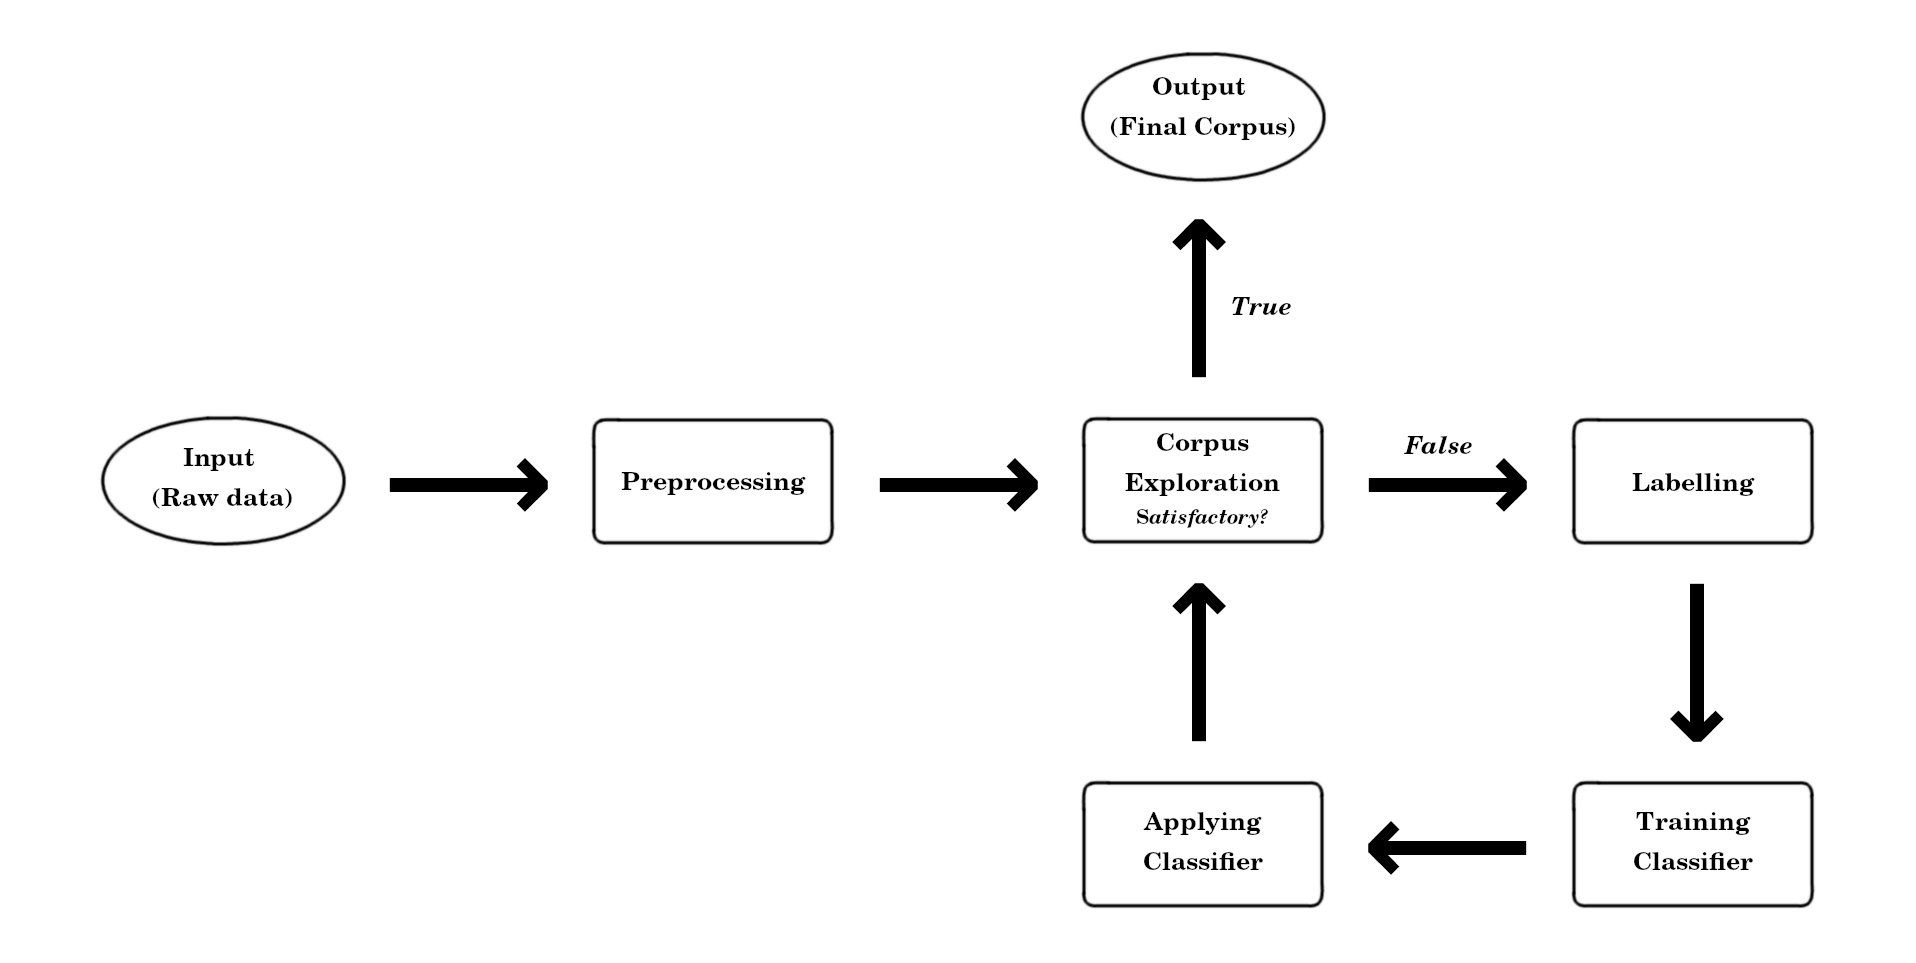
\includegraphics[width=\textwidth]{images/flow_diagram.png}
    \caption{Flow diagram of corpus construction process.}
    \label{f:flow}
\end{figure}

The process for constructing the corpus consisted of five steps (Figure \ref{f:flow}). First, a preprocessing phase, in which the XML files for the corpus were run through, divided into articles, and placed in a Pandas dataframe (\S \ref{s:preprop}). Second, exploration of the dataset to find articles of interest, using keyword searches, concordancing, collocation and co-occurrence analysis (\S \ref{s:explore}). This step merges with the third step, namely, labelling articles according to a series of hierarchical classificatory labels (\S \ref{s:labelling}). Having labelled a number of articles, we then train a naive bayes classifier using the labelled data, optimising parameters using a grid search method (\S \ref{s:nbc}). The fifth step is to apply the resulting classifier to the whole dataset. This produces a candidate corpus of relevant articles. Having reached this stage, we can return to step two to begin another iteration of the bootstrapping process.\footnote{
The term `bootstrapping' is used to indicate that earlier stages of the process are used in order to generate more satisfactory results at later stages. The process `pulls itself up by its bootstraps'. The term is widely used, with various more specific meanings, in many disciplines. One prominent example in philosophy is \cite{glymour}. The possibility of continuing to label articles and train increasingly successful classifiers can be seen in Figure \ref{f:flow} in the possibility of continually looping around the corpus exploration, labelling, training, and application phases.
}

In this project, two iterations of the process were carried out.
It is convenient to briefly characterise these iterations now before describing each part of the process in more detail. Rather than beginning with the full processed dataset, the first corpus exploration stage was started with the subset of the corpus containing regular expression matches with `philoso*'.\footnote{This matches any string which starts with `philoso', for instance, `philosophy' or `philosopher'. Code for filtering the dataset by regular expression is available in `keywords\_\-from\_\-corpus.py'. The script `multithread\_\-keyword\_\-search.py' allows for matches with regular expression search terms to be pulled directly from the dataset tarball and returned as a dataframe. This allows the user to avoid generating a dataframe for the whole dataset if it is not useful to them.  Unless otherwise stated, Python scripts and Jupyter notebooks are found in the top level directory of the project's GitHub repository at \url{https://github.com/JoshuaDavidBlack/NPOD_Philosophy}.
} We will call this corpus the Philoso* corpus. The corpus resulting from the application of the first trained Naive Bayes classifier will be called the NB1 corpus, and the corpus resulting from the second Naive Bayes classifier will be called the NB2 corpus. The sizes of these corpora are presented in Table \ref{t:corpus-sizes}.

\subsubsection{Preprocessing}\label{s:preprop}

The data processing stage begins with newspaper-year tarballs, stored in directories corresponding to each newspaper.\footnote{See `generate\_\-corpus\_\-df.py' for the full code for this step.} These were iterated through, with each tarball decompressed and each issue then processed. The METS file for each issue was first scanned, finding each item tagged 'ARTICLE' within the 'logical structure' tag. This excludes all newspaper items tagged with 'ADVERTISEMENT'.\footnote{It was decided that actual philosophical discourse is most likely to appear in full articles. However, as one of the focuses of the project is reports of public events, it is worth noting that advertisements for such events are excluded by this step. If one were wanting, for instance, to track touring public lecturers across the country, this kind of information might be worth keeping and relevant to an understanding of philosophy as it appears in this dataset. Traditional studies of newspaper reports of lectures sometimes appeal to such advertisements (e.g. \cite[fn. 13]{crane-2013} cites a lecture advertisement in the 29/06/1882 edition of the Otago Daily Times).

A more surprising instance of philosophical material appearing in advertising material is a riff on a recent lecture on evolution in the context of an advertisement a local store \cite[39--40]{crane-2013}.
}
Each `div' tag with attribute `ARTICLE' was then iterated through in order to collect the identifiers of its child `area' tags. These represent the areas of text which correspond to the article in the scans of the various pages of the issue. % say something about the process which produces these XML files?

Having collected the articles in the issue, and all of the areas of the physical pages which correspond to each issue, we then iterate through each article again, collecting the text which makes up each block. We collect these as a list of strings, where each string corresponds to an area of the page in which the article appears. In practice, each area corresponds to a paragraph of text.\footnote{These are also referred to elsewhere in the report, and exclusively in the project code, as `blocks' or `text blocks'. This is more convenient once we have abstracted away from thinking of the specific areas on a printed page.}

A unique code is assigned to each article by appending the article number from the issue to the newspaper name and date of issue. So, for instance, an article might have the code `CHP\_\-18820107\_\-ARTICLE20', which would indicate that the article comes from the issue of \textit{The Press} from the seventh of  January 1882, and that it is the 20th article as numbered in the `logical structure' contained in the issue's METS file. These codes were used to index a dataframe with the article title and article text as columns.

In order to process this large amount of data efficiently, the Python Multiprocessing library was used in order to process multiple tarballs at once. As the whole processed dataset is too large to be conveniently stored in memory, it is stored as eight pickled dataframes, compressed as .tar.gz files. These take up eight gigabytes on disk.\footnote{This reduction in size is a sign that the methods used in this project use only a small amount of the information contained in the dataset. In particular, we ignore almost all spatial information. The only exception to this is the maintenance of distinct blocks of text.}

\subsubsection{Dataset Exploration}\label{s:explore}

\begin{table}[]
        \centering
        \begin{tabular}{l|c}
             Corpus &  Article Count \\
             \hline
          Processed dataset & 7592619 \\
          `philoso*' Corpus &	29647 \\
          Naive Bayes 1 &	239649 \\
          Naive Bayes 2 & 31131
        \end{tabular}
        \caption{Article counts for processed dataset and general philosophy corpora.}
        \label{t:corpus-sizes}
\end{table}

The purpose of the exploration phase of the process is to determine the nature of the current candidate corpus and to pick out any keyword or articles which are good candidates to be labelled and used to train a classifier. This section sets out some of the main tools used at this stage. The techniques discussed here are, in order, manual inspection of the articles in the developing corpus, concordancing, collocation analysis, and co-occurrence networks.

Manual inspection of a random subset of a corpus indicates the general kind of material it contains. This might also reveal anything \textit{missing} from the corpus. Inspection of the Philoso* corpus revealed plenty of material of the desired sort, including reports of public events (e.g. `CHP\_\-18690823\_\-ARTICLE15', on a lecture against Darwinism on the grounds that it goes beyond claims that can be made by the sciences); letters to the editor (e.g. `CHP\_\-18920926\_\-ARTICLE10'); and first-order philosophical writing (e.g. `CL\_\-18790919\_\-ARTICLE27').\footnote{See the notebook `philoso\_\-subset\_\-exp.ipynb' for full code for the exploratory steps using the Philoso* corpus.} It was also found to contain various material which we are not interested in. For instance, pieces of serialised fiction which describe a character as `phliosophical' but don't engage in philosophical discourse (e.g. `GLOBE\_\-18770315\_\-ARTICLE12'); or use of the word `philosophical' to mean indifferent or resigned (e.g. `OW\_\-18920721\_\-ARTICLE7').

\begin{table}[]
        \footnotesize
        \centering
        \begin{tabular}{l|lcr}
        1 & n with tho university a chair of logic moral & philosophy & and political economy ah along tho church ha \\
        2 & own god the cause of ' all causes before all & philosophy & before all systems creeds and divinations be \\
        3 & elves to the dangerous charm of specula live & philosophy & and drifting far away from the safe anchorag \\
        4 & heaven and earth than are dreamt of in their & philosophy & and if' we should only discover one or two o \\
        5 & ish as to try to estab lish a chair of moral & philosophy & in seaeliff as you will observe sir mr adams \\
        6 & se you and he had last evening about natural & philosophy & ' 'no ghosts ' answered la dy cecil gravely \\
        \end{tabular}
        \caption{Selected results from `philosophy' concordance.}
        \label{t:corpus-concordance}
\end{table}

To obtain a `more distant' view of the content of the corpus, concordancing was carried out using the NLTK package \cite{bird-2009}. An entry of a concordance is an occurrence of a given word in context within the corpus. A selected subset of concordance results for `philosophy', within the Philoso* corpus, is presented in Table \ref{t:corpus-concordance}. We see reference to academic philosophy in (1) and (5); religious involvement in (1) and (2); something which looks like fiction in (6); the idea of philosophy as dangerous in (3); and the use of a well-worn phrase from Hamlet in (4). We also see some of the shortcomings of the OCR, with lots of word breaks present where they should not be and missed letters. For instance, `seaeliff' should be `seacliff' in (5).

\begin{table}[]
        \footnotesize
        \centering
        \begin{tabular}{l|l}
          Rank & Collocation  \\
          \hline
        1 & ('philosophy', 'reflectiveness') \\
        2 & ('synthetic', 'philosophy') \\
        3 & ('dreamt', 'philosophy') \\
        4 & ('undreamed', 'philosophy') \\
        5 & ('baconian', 'philosophy') \\
        6 & ('undreamt', 'philosophy') \\
        7 & ('proverbial', 'philosophy') \\
        8 & ('epicurean', 'philosophy') \\
        9 & ('philosophy', 'apparel') \\
        10 & ('axioms', 'philosophy') \\
        11 & ('matics', 'philosophy') \\
        12 & ('inductive', 'philosophy') \\
        13 & ('cosmic', 'philosophy') \\
        14 & ('foregoing', 'philosophy') \\
        15 & ('transcendental', 'philosophy') \\
        \end{tabular}
        \caption{Top 15 Collocations with `philosophy', window size of 5, ranked by pointwise mutual information.}
        \label{t:corpus-collocation}
\end{table}

Collocation analysis also suggested a large amount of relevant material. A collocation is a word whose appearance within a given distance from a search term is significant. The selected window size for collocations with `philosophy' was five to the left and right of the word. The significance of  collocations was ranked by pointwise mutual information score. This, informally speaking, ranks the pair by how much information is given about the occurrence of one word given the appearance of the other. In Table \ref{t:corpus-collocation}, we see philosophy associated with reflection in general in (1); apparent references to the Hamlet quote above in (3), (4), and (6); reference to the sciences in (12); particular schools of philosophy (5) and (8); and some more confusing entries, e.g. (9).

The final exploratory method applied was co-occurrence network analysis. Unlike collocations, which must appear within a window of a given word, we calculated document-level co-occurrence statistics. The approach followed in this project is derived from \cite{cooccurrence-tutorial}, with modifications to convert the approach from R to Python. Co-occurrence statistics were computed with Numpy \cite{harris2020array}, and visualised as networks using Dash cytoscapes \cite{plotly}. In addition to mutual information, co-occurrence scores were calculated with the `log Dice' metric, which is designed to be consistent across different corpus sizes and insensitive to word frequency \cite{logdice}.\footnote{The calculation of log dice and mutual information co occurrences are done by the functions `log\_\-dice\_\-coocs' and `mi\_\-coocs' respectively, while the construction of the co-occurrence network is performed by the function `network\_\-dash'. All three are in the file `NL\_\-helpers.py'. The Dash visualisation code is most easily inspected within the GitHub repository for the Heroku dashboard at \url{https://github.com/JoshuaDavidBlack/NPOD_Philosophy_Heroku}.}

One issue which arises for co-occurrence analysis is the creation of an appropriate dictionary. This is especially important for a large corpus generated by OCR. In such cases, automatic generation of a dictionary is likely to result in a large collection of non-words. A few approaches were used to avoid this. Using the Gensim package \cite{gensim}, it was specified that a word must appear in more than 20 articles and in less than 40\% of articles in order to appear in the dictionary.\footnote{This code is also contained in `philo\_\-subset\_\-exp.ipynb'.} In addition, the tokenised text was further filtered to only include words which appear in the NLTK English words dictionary.\footnote{The `wordlist' corpora was used, corresponding to the `/usr/share/dict/words' file on Unix systems. See Chapter 2 of \cite{bird-2009}.}
The number of resulting words in the dictionary varied by corpus, but this kind of filtering was sufficient to enable the calculation of collocation scores without overwhelming available memory resources. The main constraint here is the size of the `document-term matrix' and `term-term matrix' required to calculate the co-occurrence scores. The former is a dictionary size by number of documents matrix containing the number of occurrences of each word in each document, and the latter is a dictionary by dictionary size matrix containing how often a given term appears in a document with another.\footnote{Code to generate these matrices is included in `Entity Extraction with Philo Subset.ipynb', `generate\_\-matrices\_\-propn.py', and `generate\_\-matrices\_\-entities.py'.}

One downside of this method of filtering is that the names of entities which appear in the dataset, but which do not appear in an English dictionary, are lost.\footnote{While the wordlist corpus used as an English dictionary has many names, it does not have \emph{all} names.} This is particularly worrying for the historian of philosophy, who may want to pick out particular people or institutions to be the subject of further research. To overcome this problem, two further dictionaries we made by  running the corpus through SpaCy \cite{spacy} to pick out both named entities and proper nouns.\footnote{See code in, e.g, `Entity Extraction with Philoso Subset.ipynb'.} These were then ran as through the same dictionary creation approach as described above.

Co-occurrences were calculated using both the Bag of Words and TF-IDF transformation representations of the documents. The TF-IDF transformation scales word scores both on the basis of the number of words in the given article and the frequency of the given word in the corpus. This was also done using the Gensim package.

\begin{figure}
    \centering
    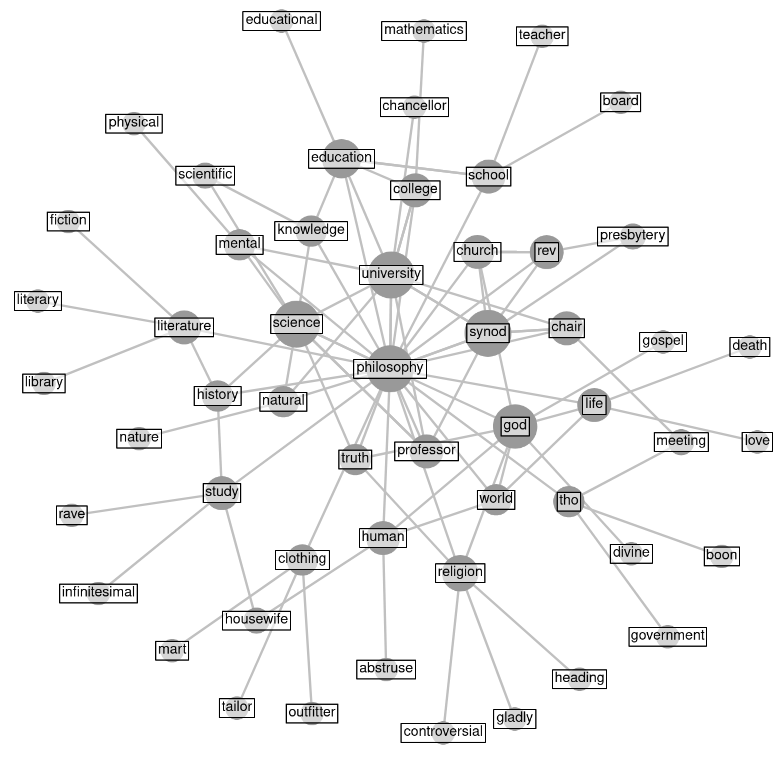
\includegraphics[width=0.8\textwidth]{images/philo_cooccurrence.png}
    \caption{Co-occurrence network for `philosophy' in Philoso* corpus, with TF-IDF transformation, and Log Dice statistic. The top 25 co-occurrences for `philosophy' are shown, with the four top co-occurrences for each of these words also added to the network.}
    \label{f:cooccurrence}
\end{figure}

Figure \ref{f:cooccurrence} provides an example of a co-occurrence network generated during the first stages of the corpus construction process.\footnote{Many more such networks can be produced using the dashboard at \url{http://nz-newspaper-philosophy.herokuapp.com}.}. The width of the edges indicate the strength of co-occurrence and the size of the nodes indicates the number of connections the node has. The figure shows the close connections of philosophy both with the academic word and also with church bodies (see, e.g. `synod'). There are some surprising words included as well, for instance, `clothing'.\footnote{Looking in to this, it seems that an advertisement referring to the `philosophy of clothing' appended to the end of articles for a clothing company in the \textit{Daily Sourthern Cross} is responsible for this connection, e.g. \cite{clothing-example}. This may also explain the confusing entry `apparel' in the collocation results in Table \ref{t:corpus-collocation}.}

\subsubsection{Labelling Articles}\label{s:labelling}

Each of the exploratory steps set out above helped to clarify what kind of philosophical writing we could expect to find, and what kind of material we want to exclude. This understanding enabled the creation of a collection of labelled articles, stored as a Pandas dataframe.\footnote{The notebook `Classifying texts.ipynb' contains code used to label articles.}  All labelling was carried out at the article level and relied on the investigator's experience in research in the history of philosophy.\footnote{The investigator has a PhD in Philosophy focusing on a particular figure in late nineteenth century philosophy.} This puts it in the category of single-annotator corpora rather than those whose labels have been validated by multiple investigators. Five labels were used.

\begin{table}[]
        \centering
        \footnotesize
        \begin{tabular}{l|ll|ll}
          & \textbf{First Iteration} & & \textbf{Second Iteration}  & \\
          Label & Value & Count & Value & Count \\
          \hline
          & & & &  \\
        	Readable & True & 247 & True & 918 \\
        	& False & 26 & False & 41 \\
          & & & &  \\
          Philosophy & True & 101 & True & 299 \\
          & False & 147 & False & 620 \\
          & & & &  \\
          Philosophy Type & Religion-Science & 58 & Religion-Science & 140 \\
          & Ethics-Politics & 25 &  Ethics-Politics & 94 \\
          & Epistemology-Metaphysics & 3 & Epistemology-Metaphysics & 13 \\
          & Other & 15 &  Other & 52 \\
          & & & &  \\
          Writing Type & Public Event & 40 & Public Event & 97 \\
          & Letter to the Editor & 23 &  Letter to the Editor & 69 \\
          & First-order Writing & 36 &  First-order Writing & 111 \\
          & Review & 2 &  Other & 22 \\
          & & & &  \\
          NZ & True & 77 & True & 178 \\
          & False & 12 & False & 41 \\
        \end{tabular}
        \caption{Label counts before first classifier was applied (First Iteration) and the second classifier was applied (Second Iteration).}
        \label{t:labels}
\end{table}

The first label tracks whether an article is readable or not. The criterion for readability was whether the investigator could decipher the sentence without any appeal to the original image. The methods used later in the project use bag of words representations of the texts. Such methods do not rely on having high quality sequences of text. If the investigator was able to pick out from the features on the page that the article is relevant, it is hoped that the features used by the classification and topic modelling algorithms are also sufficient to pick out the article. In any case in which a user of the corpus is interested in a text which is too garbled to read, enough information is provided for the user to access to the original scan from the Papers Past website and correct the OCR. The readability label is stored as a boolean for all articles in the labelled collection.

The second label tracks whether something is `philosophy' or not. The criterion for inclusion was, as suggested by the characterisation of `philosophical discourse' in Section \ref{s:project-motivations}. If the investigator judged that `ultimate values' or `ultimate reality' were being discussed, the article was included. Pieces discussing the practice of philosophical reflection were also included, for instance, material about philosophy provision at the universities. The philosophy label is stored as a boolean for all articles in the labelled collection.

An problem which had to be solved while labelling philosophy articles was the presence of large editorial articles in which multiple subjects are discussed in turn. In such articles, a report on a local fire, a reflection on some philosophical topic, and a bit of society gossip might all be put together. For instance, the article with code 'AS\_\-18860821\_\-ARTICLE40' consists of 28 blocks, of which 5 are dedicated to an argument with a reader over whether suicide is ethical \cite{suicide-example}. These five blocks are definitely `philosophical discourse', but the remaining blocks discuss poetry, a local operatic production and the close of a sitting of parliament. In the current version of the labelled dataframe, many such `composite' articles are included.\footnote{This is discussed again in Section \ref{s:corpus-results} and Section \ref{s:discussion}.}

The next label tracks the genre of philosophy present in the article. The two main labels for this were `r', indicating a discussion of religious belief and its relationship to modern science, understood widely to include the natural sciences, history, and biblical criticism; and `e', indicating a discussion of ethics or politics. The label `m' was used for metaphysics and epistemology and the label `o' was used for `other'. The metaphysics and epistemology label was designed to be used for purely secular discussion of, e.g., the nature of knowledge or reality. One could, for instance, discuss whether free will is possible given modern scientific results without discussing anything directly to do with religion. However, in practice, almost all discussions of these topics were more readily labelled with `r'. This label falls under the philosophy label. That is, only those article labelled as philosophical have a `philosophy type' label.

The fourth label was `writing type'. This has three values: `l' indicates a letter to the editor of the newspaper; 'p' indicates a report of a public event, such as a debate, lecture or sermon; `f' indicates a first-order piece of philosophical discourse and `r' indicates a book review. Only articles labelled with `philosophy' were labelled with a writing type. However, this restriction was unnecessary and indeed not helpful if one were to try to train an algorithm to distinguish these writings types. In a future version of the project non-philosophy lectures and letters to the editor should also be labelled.

The final label was `NZ', which tracks whether the author of the piece is based in New Zealand or not. In practice, almost all articles are tagged as being written by a New Zealand-based author. It was hoped that this tag might help with investigating the `New Zealandness' of the corpus. However, this was abandoned as the lack of clearly `non-New Zealand' pieces made it seem implausible that a useful classifier could be trained. The labelled collection also contains any notes which might be relevant to the decision or be interesting to future researchers. Only articles labelled as philosophy and for which the investigator could determine authorship were labelled with an `NZ' label.

Philosophy articles were found by a few methods. First, some of the articles found in initial exploration of the dataset were added. Second, keyword searches using the results of the more formal exploration set out in the previous section were used. For instance, keyword searching for interesting collocates and co-occurring terms of `philosophy'. This second step found many non-philosophy articles as well. In addition, a random sample of the processed dataset was passed to the labelling stage, to ensure a broad range of non-philosophy articles were included.

The distribution of labels in the labelled collection is presented in Table \ref{t:labels}.\footnote{The version of the labelled dataset used for the first iteration is stored as a pickled Pandas dataframe at `pickles/classifier\_\-with\_\-text\_\-nb1.pickle'. The version of the dataset used for the second iteration is contained in `pickles/classified\_\-with\_\-text\_\-df.pickle'.} Note that it is harder to find philosophy articles than non-philosophy articles even when using keyword searches and the exploratory methods set out above. Most articles labelled were readable, and the various writing types were well represented. As noted above, the epistemology-metaphysics label was not used much. Note that material focused on religion is very prominent in the dataset in general and this is carried in to the labelled collection.

\subsubsection{Naive Bayes Classification}\label{s:nbc}

Having labelled a set of articles, a classification algorithm was trained. The only label used for the purpose of creating a corpus of philosophical discourse was the `philosophy' label.\footnote{An attempt to produce a `readability' classifier to run before classifying between philosophy and non-philosophy. This is present in `NaiveBayes\_\-PhilosophyClassification\_\-SecondSet.ipynb'. Good performance was not attained. In practice, almost all non-readable articles are classifier as non-philosophy by the philosophy classifier.}
 At each training stage, the labelled collection was divided into testing and training sets. In the first iteration of the process, the philosophy articles were divided, with 75 in the training set and 26 in the test set.\footnote{The code for the first iteration is found in the notebook `NaiveBayes\_\-PhilosophyClassification.ipynb'.}
The training set contained 75 of the non-philosophy articles and test set contained the remainder of the non-phliosophy articles. This was done in order to ensure a 50/50 class balance in the training set, while the higher proportion of non-philosophy in the test set more closely matches the real situation in the dataset as a whole.\footnote{In fact, the test set massively over-estimates the amount of philosophical discourse in the dataset as a whole. For this reason, it was not considered important to follow the usual practice of handling class balance \emph{after} the split between testing and training data.}

In the second iteration of the process, the training set was assigned 75\% of each of the philosophy and non-philosophy articles (222 and 465 articles respectively).\footnote{Code for classifier training in the second iteration is found in the notebook `NaiveBayes\_\-PhilosophyClassification\_\-SecondSet.ipynb'.} The remainder of articles were assigned to the test set. To achieve a closer class balance in the training set, random upsampling was applied to the philosophy articles. This was done by randomly doubling a sample of between 20 and 50 philosophy articles, and repeating the process until there were 407 articles assigned to philosophy in the training set.\footnote{The increase in the proportion of non-philosophy in the labelled data in the second iteration meant that it was more convenient to use the usual approach of first dividing the test and training before dealing with class balance.}

The Scikit-learn package was used to implement classification algorithms \cite{scikit-learn}. The pipeline takes the text and converts it into a bag of words representation, implements a TF-IDF transformation, and then feeds the result into a Naive Bayes classifier.

The Naive Bayes classifier was adopted on the basis that it is a simple and easy to train model which performs surprisingly well at text classification \cite{zhang-2004}.\footnote{The use of a Support Vector classifier rather than Naive Bayes was considered, but no improvement on the Naive Bayes approach was found. This is further discussed in Section \ref{s:alternative-classifiers}.} The naive in `Naive Bayes' indicates that the algorithm treats each of the features fed to it as probabilistically independent. This is obviously not true of our dataset in reality. The appearance of a given word will definitely affect the probabilities of the other words in the dictionary appearing in any case of real writing.\footnote{Strictly, it assumes all features are independent conditional on the class to which the object is assigned. That is, that, e.g., the probability of the appearance of 'Darwinism' given that the article is a philosophy article is independent of the probability that `evolution' appears given that the article is a philosophy article. This is similarly implausible.} This was a particularly appropriate choice given the lack of high-quality sequence data noted above. Naive Bayes operates on a bag of words representation of the document. % Say something about speed?

In order to determine the optimal parameters for this pipeline, a grid cross validation approach was used. The parameter space considered for each iteration of the process is presented in Table \ref{t:CV}, along with the parameters values chosen. In both cases, the training set was divided into five for cross validation. Overall accuracy was used as the cross-validation metric. Precision and recall were also tried as metrics, but balancing the two with overall accuracy seemed to work best. The model selected using overall accuracy does not suffer from either low recall or precision. This will be further discussed in the results section (\S \ref{s:corpus-results}).

\begin{table}[]
        \centering
        \footnotesize
        \begin{tabular}{l|ll|ll}
           & \textbf{First Iteration} & & \textbf{Second Iteration} & \\
          Parameter & Range & Selected & Range & Selected \\
          \hline
          Minimum documents (count) & 5-12 & 7 & [2, 5, 7, 10, 15] & 2 \\ %This doesn't look good. Fix if you get a chance. Check!
          Maximum documents (prop) & 0.2-0.5 & 0.2 & 0.2-0.6 & 0.4 \\
          N-gram range & (1,1)-(1,3) & (1, 1) & (1,1)-(1,3) & (1, 1) \\
          TF-IDF & True/False & True & True/False & True \\
          Stopwords & incl. 'philosophy' (True/False) & False & N/A & N/A \\
          Smoothing parameter& N/A & N/A & [0.5, 0.75, 0.1] & 0.5
        \end{tabular}
        \caption{Cross Validation Parameter Space and Selected Value.}
        \label{t:CV}
\end{table}

The majority of the parameters selected for the purpose of the search concern the preprocessing of the articles fed to the classifier. The minimum number of documents containing a given word and the maximum proportion of documents containing it both control the words which are included in the dictionary used by the classifier. The n-gram range allows for collections of words of length up to three to be considered by the classifier. The TF-IDF transformation has been noted above. It controls for the length of documents and the prevalence of words in the corpus as a whole. In the first iteration, the addition of `philosophy' to the stop words was considered, as the `philoso*' corpus was thought to over-emphasise the word. This was abandoned at the second iteration.

Three values of smoothing parameter were considered in the second iteration. A smoothing parameter adds a `pseudocount' to each of the words in the dictionary to account for the difference between the particular distribution of words in the articles given to the classifier and the real distribution. For instance, it may be that no articles labelled as philosophy in the training data contain the word `dog'. We would not want to conclude from this that the probability of an article containing `dog' being philosophy is zero. Consequently, a `smoothing' value is added to the count to ensure that the probability of any word appearing in a given class is non-zero. The smaller this value is, the closer we are taking the distribution of the articles in the dataset and in the real world to be. One risk is that, if we set this too low, the classifier will over fit the training data. Consequently, values below 0.5 were not allowed.

\subsubsection{Classifier Application and Bootstrapping}

In order to `bootstrap', once a classifier was selected, it was applied to the entire dataset of newspaper articles, and dataframe resulting from keeping the articles classified as `philosophy' was pickled. At this point, another round of corpus exploration and labelling could be carried out. If the result is considered satisfactory after exploration, the corpus construction phase is considered to be over.

The motivation for going around another labelling and training loop is that the labelling the non-philosophy picked out from the dataset by an earlier classifier enables later classifiers to more accurately select the relevant material from the dataset. The involvement of the investigator in selecting and labelling everything which goes in to the labelled collection ensures that we don't have a `garbage in - garbage out' problem, which might occur if poor results of a previous classifier were directly fed in to later stages. That is, we don't need to worry that bootstrapping will result in articles in the labelled collection as `philosophy' which are not really philosophy articles. On the other hand, if an early classifier excludes a lot of philosophy articles, then the process outlined in Figure \ref{f:flow} will struggle to find them. To overcome this, effort to get a wide range of philosophy in the labelled collection before training the first classifier is important.

\subsection{Implementation}\label{s:corpus-implementation}

This section contains some brief notes on the implementation of the above methods.

\subsubsection{Hardware and Multiprocessing}\label{s:corpus-implementation-multi}

The project has been almost entirely carried out on a workstation PC with a AMD Ryzen Threadripper 1950X 16-Core Processor with 32 threads and 32GB of RAM. This setup conditioned the code written for the project in a two main ways.

Firstly, the Python multiprocessing module was used to enable more than one thread to be used at once. This was particularly important for operations involving the whole dataset. Being able to open and process 16 tarballs at once was significantly more efficient than opening one at a time.

Secondly, limitations in RAM required the dataset to be sliced into very small subsets to enable models to be fit to the whole corpus efficiently. Around 70 slices were used, and stored on an SSD to enable faster I/O. This allowed for multiple cores to fit a trained model without having to open up multiple very large slices of the dataset. Similarly, the corpus produced by the first classifier (around 200,000 documents) needed to be reformatted to allow it to be run through a topic modelling algorithm without overrunning the available RAM. This was done by storing the bag of words representation of each document in a `.csv' file on the SSD and feading these documents one at a time to the algorithm without loading the whole corpus into RAM.\footnote{See, especially, the class `NL\_\-streamed\_\-corpus' in the file `NL\_\-topicmodels.py'}

\subsubsection{From METS/ALTO to Pandas}

The tarballs for two years of the \textit{Lyttelton Times}, 1890 and 1891, were corrupted and have been excluded. This is not important for the humanities questions investigated in the following section, but would be if one were trying to compare the number of philosophical articles in different newspapers in aggregate or over time.

A small number of individual issues of newspapers were also excluded on the basis of problems with parsing their ALTO/METS XML. This problem only appeared for a handful of issues, and so has been ignored. Manual inspection also suggests that some articles have also got missing blocks. This is unlikely to be important in the aggregate.

\subsubsection{Dashboard Construction: Dash and Heroku}

The dashboard available at \url{https://nz-newspaper-philosophy.herokuapp.com} is hosted on their `hobby' service and lacks the power to directly compute anything from the corpora available to it. Consequently, precomputed results for various search terms have been added in the form of small dataframes.\footnote{A Dash cytoscape interface which enables the user to enter their own search terms is available in `Religion and Evolution in the Rel corpus.ipynb'. This can be run on the users own computer, rather than on the Heroku server.}

\subsection{Results}\label{s:corpus-results}

\subsubsection{Classification Metrics}\label{s:classification-metrics}

Both the first and second classifier have very similar overall accuracy on their respective test sets. With 0.90 for the first classifier and 0.89 for the second classifier. Confusion matrices for these classifiers are presented by Table \ref{t:nb1-confusion} and Table \ref{t:nb2-confusion}.

\begin{table}[]
        \centering
        \footnotesize
        \begin{tabular}{ll|ll}
        & & \textbf{Predicted} & \\
        & & False & True \\
        \hline
        \textbf{Actual} & False & 88 & 9 \\
        & True & 3 & 23 \\
        \end{tabular}
        \caption{Confusion Matrix for First Naive Bayes Classifier}
        \label{t:nb1-confusion}
\end{table}

This may make it sound like future iterations made the performance of the classifier worse. However, a straightforward comparison between the numbers is not appropriate. The second classifier had many more non-philosophy articles in its test set than the first. Moreover, it was given much finer distinctions than the first classifier. That is, the second classifier had a lot more non-philosophy which looked similar to the desired philosophy articles than did the first classifier. This is because of the `bootstrapping' approach, where the NB1 corpus was used a source of new articles for labelling. Given this, many of the non-philosophy articles given to the second classifier were articles that were labelled as philosophy by the first.

\begin{table}[]
        \centering
        \footnotesize
        \begin{tabular}{ll|ll}
        & & \textbf{Predicted} & \\
        & & False & True \\
        \hline
        \textbf{Actual} & False & 181 & 14 \\
        & True & 15 & 62 \\
        \end{tabular}
        \caption{Confusion Matrix for Second Naive Bayes Classifier}
        \label{t:nb2-confusion}
\end{table}

Overall accuracy is not the only relevant metric for a binary classifier. The confusion matrices for the two classifiers suggest that a reasonable balance between recall and precision is being achieved. In the case of the first Naive Bayes classifier, we have a recall of 0.88, and a precision of 0.71. In the case of the second Naive Bayes classifier we have a recall of 0.80, and a precision of 0.81. These figures show, at least, that accuracy is not being attained at the expense of either precision or recall.

Another way to consider the difference is to look at the size of the resulting corpora. Applying the first classifier results in a corpus with around 200,000 articles, whereas the applying the second results in a corpus with around 30,000 articles (see Table \ref{t:corpus-sizes}). This shows that the second classifier is at least picking out a smaller proportion of articles to tag as philosophy. However, to determine whether the articles picked are actually the articles which are desired, it will be necessary to turn to more direct inspection of the resulting corpus.

\subsubsection{Manual Inspection of False Positives and Negatives}

There are two aspects of classifier performance to manually check and apply qualitative judgement to. First, the false positives and negatives when the classifier is applied to the test set. Second, the composition of the corpus which results from applying the classifier to the whole dataset. The false positives and false negatives picked out by the second Naive Bayes classifier will reveal how the classifier is erring on the labelled collection and reveal what kind of articles we should expect to get into the corpus generated by applying the classifier to the entire dataset.\footnote{We could also consider those articles which are misclassified in the training set. However, for the purposes of getting an idea of the general kind of articles that will be misclassified, the test set should be sufficient.}

\begin{table}[]
        \centering
        \footnotesize
        \begin{tabular}{l|l}
          Category & Count \\
          \hline
          Composite pieces & 4 \\
          Ethics (correctly labelled) & 7 \\
          Ethics (mislabelled) & 3 \\
          Other (correctly labelled) & 1\\
          Other (mislabelled) & 0 \\
          \textbf{Total} & 15\\
        \end{tabular}
        \caption{Categorised false negatives for second Naive Bayes classifier.}
        \label{t:false-negatives}
\end{table}

Table \ref{t:false-negatives} presents the false negatives when the second classifier was applied to the test set.\footnote{See Table \ref{t:false-negatives-full} for a full list.} Note the presence of four composite pieces. These are pieces where only a small section is `philosophical'.\footnote{As discussion earlier (\S \ref{s:labelling}).} Note also that the majority of the false positives come from the `ethics' category, which covers both personal ethics and political issues. Three of these can, on reflection, be seen to be mislabelled. Usually, this is because they only make a passing reference to philosophy, rather than engaging in any philosophical discourse.\footnote{DTN\_\-18940820\_\-ARTICLE7, for instance, mentions the philosopher John Stuart Mill in passing, but is not otherwise philosophical.} %Change to proper reference if you get the time.

The false negative results suggest that the classifier is struggling to capture ethics and politics, but not struggling with religious material. They also highlight shortcomings in the labelling scheme adopted in this project. Section \ref{s:discussion} will discuss possible improvements to the handling of both composite pieces and the ethics category.

\begin{table}[]
        \centering
        \footnotesize
        \begin{tabular}{l|l}
          Category & Count \\
          \hline
          Mislabelled (religious) & 3 \\
          Correctly labelled (religious) & 5\\
          Edge case (religious) & 2 \\
          Correctly labelled (other) & 3 \\
          Unreadable & 1 \\
          \textbf{Total} & 14
        \end{tabular}
        \caption{Categorised false positives for second Naive Bayes classifier.}
        \label{t:false-positives}
\end{table}

Table \ref{t:false-positives} presents the false positives when the second classifier was applied to the test set.\footnote{See Table \ref{t:false-positives-full} for a full list.} Where the false negatives are dominated by ethics and politics, the false positives are dominated by religious material. This indicates that the classifier is tending to pick out the desired religious material much better than the desired ethical material. Even so, some cases are, on reflection, either difficult to say whether they ought to have been labelled as philosophy or probably should have been labelled as philosophy.\footnote{For instance, one of the edge cases is a report of a public meeting of a group called the White Cross Society, dedicated to improving local moral standard. There are, in the course of a long report, \emph{some} gestures towards the `ultimate' reasons for adopting their preferred moral framework. This will be discussed again when we return to the question of labelling (\S \ref{s:discussion}).} This, as in the case of the false negatives, indicates that the problems for the classifier are in regions where the human labelling of the dataset is also  slightly ambiguous. Of the non-religious material, we have a bit of materials science, a list of graduates of Canterbury College and their subjects, and a quack advertisement concerning the `philosophers stone'. In the latter case, the use of philosophical jargon explains how it gets misclassified, while the other two cases are at least \emph{intellectual} material if they are not philosophical.

\subsubsection{Inspection of Resulting Corpora}

Inspecting the corpora produced by running the Naive Bayes classifiers on the complete dataset encourages the idea that a sensible subset of the dataset is being picked out.\footnote{Random samples of 500 articles from each of the corpora derived in this project can be explored at \url{https://nz-newspaper-philosophy.herokuapp.com/}, using the `View Texts' tab.} For the purpose of this report, a useful way to summarise the content of each corpus is the word cloud.

Figures \ref{f:wc-corpus-10k} to \ref{f:wc-nb2} display word clouds for a subset of 10000 articles of the original dataset, the `philoso*' corpus, the corpus resulting from the first Naive Bayes classifier, and the corpus resulting from the second Naive Bayes classifier. Each of these word clouds was generated using the TF-IDF transformation and with dictionaries excluding any word which appeared in more than 20\% of the documents and less than 50 documents in total.\footnote{Word clouds were produced using the Python `wordcloud' package \cite{wordcloud}. See `generate\_\-word\_\-clouds.py'.}

\begin{figure}
  \centering
  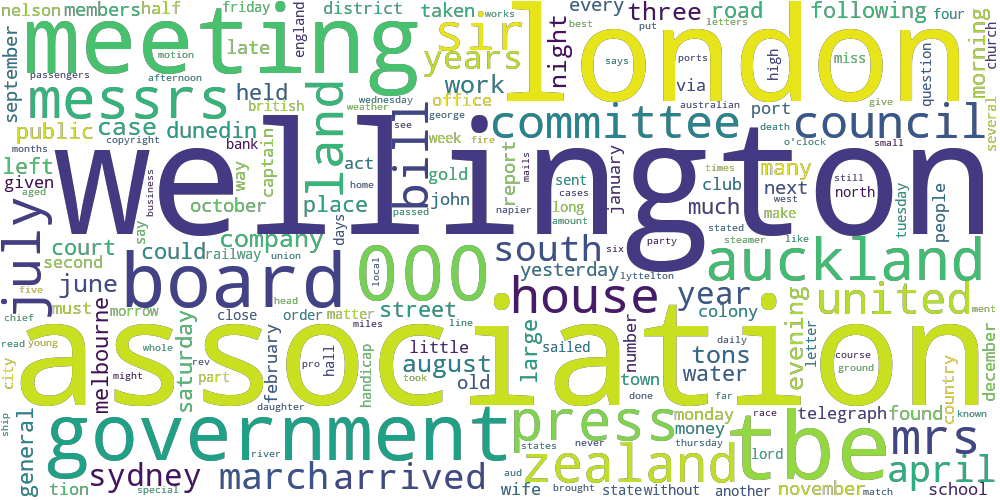
\includegraphics[width=0.9\textwidth]{images/corpus_10000_subset_tf-idf.png}
  \caption{Word cloud for random sample of full dataset.}
  \label{f:wc-corpus-10k}
\end{figure}

We see in Figure \ref{f:wc-corpus-10k}, that no particularly `philosophical' terms are present. The majority are place names, notably Wellington and London, along with terms for reporting on government, business and transportation. Figure \ref{f:wc-philoso} looks quite different, although place names are still prominent. It is particularly interesting that `women' and `miss' become very prominent. The prominence of God is also striking, and is in line with the observation that religious matters are closely intertwined with philosophy in this corpus in general.

\begin{figure}
  \centering
  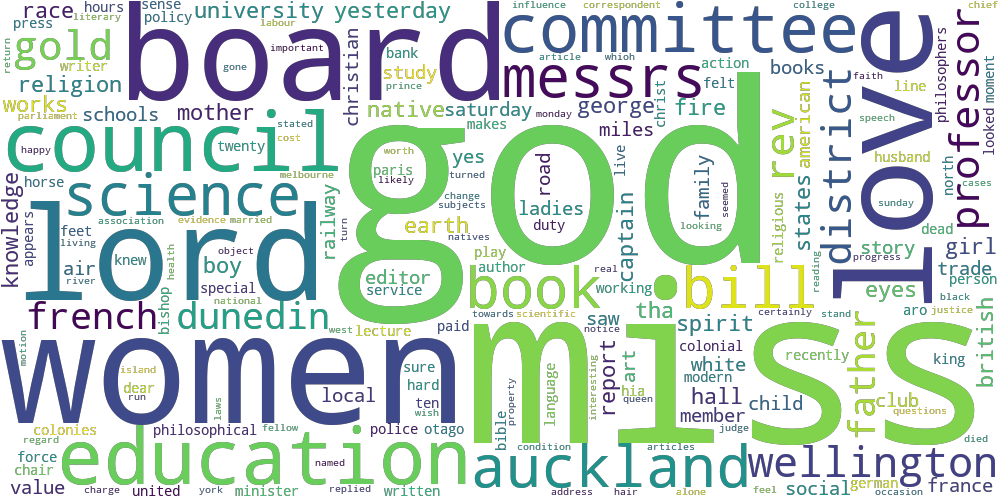
\includegraphics[width=0.9\textwidth]{images/philoso_tf-idf.png}
  \caption{Word cloud for random sample of Philoso* corpus.}
  \label{f:wc-philoso}
\end{figure}


\begin{figure}
  \centering
  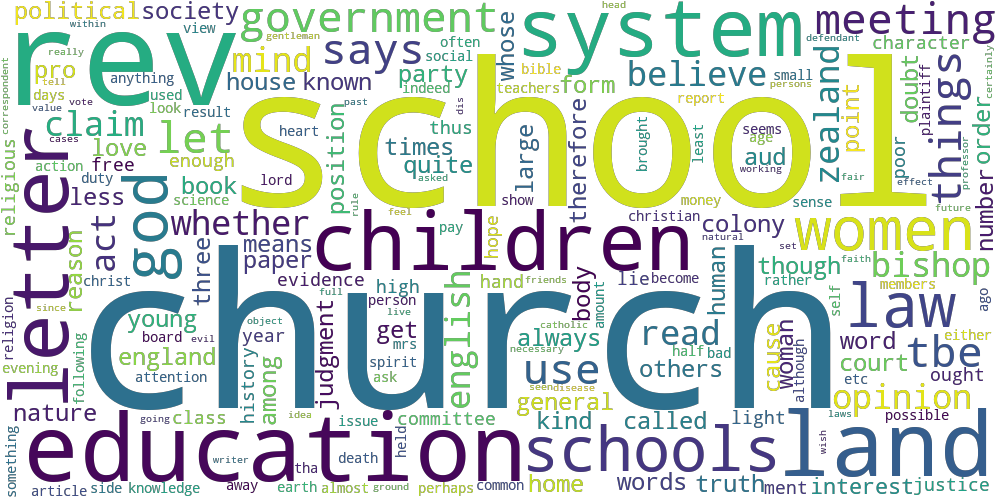
\includegraphics[width=0.9\textwidth]{images/nb1_philoso_tf-idf.png}
  \caption{Word cloud for random sample of the NB1 corpus.}
  \label{f:wc-nb1}
\end{figure}

The shift to the NB1 corpus (Figure \ref{f:wc-nb1}) increases the prominence of language about education, we also see words like `judgement' and `evidence'. This indicates the selection of intellectual content from the dataset as a whole. Finally, we see in Figure \ref{f:wc-nb2}, that education and religion maintain prominence, while words like `lecture' and `professor' start to come through. This way of summarising the content of the corpora suggests that the methods deployed here are successfully picking out a meaningful subset of the original dataset which is of intellectual interest.

\begin{figure}
  \centering
  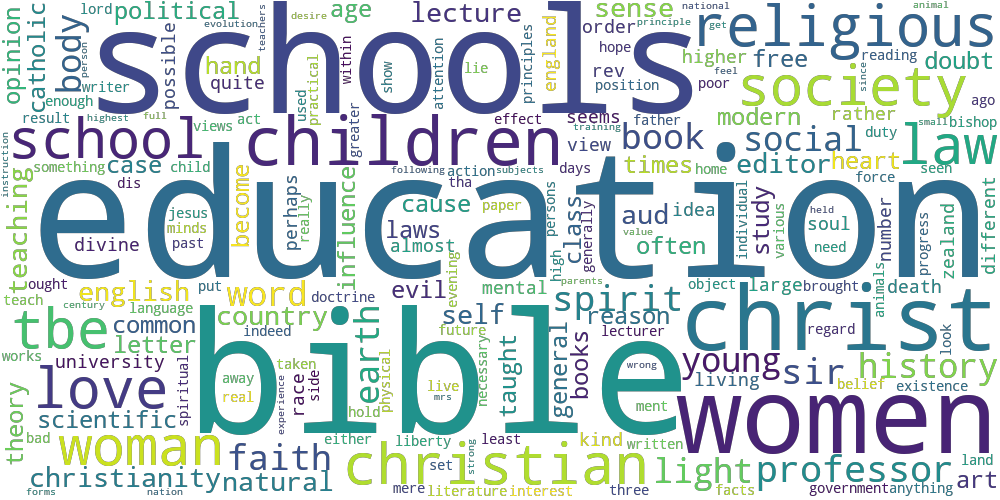
\includegraphics[width=0.9\textwidth]{images/nb2_v2_philoso_tf-idf.png}
  \caption{Word cloud for random sample of the NB2 corpus.}
  \label{f:wc-nb2}
\end{figure}


A slightly more sophisticated way of summarising the material contained in the various corpora we have considered is to run Latent Dirichlet Allocation (LDA) topic models on each.\footnote{
See `subset\_\-topicmodels.py' for details of these models.
} Table \ref{t:ten-topic} presents the results of applying a model with ten topics to the Philoso*, NB1 and NB2 corpora.

\begin{table}[]
        \centering
        \begin{tabular}{p{0.01\linewidth}|p{0.28\linewidth}| p{0.28\linewidth}| p{0.28\linewidth}}
          & \textbf{Philoso*} & \textbf{NB1} & \textbf{NB2}
          \\ \hline
          1 & young, think, mrs, lady, came, eyes, thought, woman, back, miss	& claim, judgment, plaintiff, land, defendant, costs, amount, case, sheep, pay & lecture, lecturer, subject, professor, evening, last, christianity, audience, might, lectures \\
          2	& lie, case, court, evidence, tin, law, judge, tlie, prisoner, jury & case, letter, sir, editor, say, said, law, question, matter, could & science, nature, tho, evolution, human, thought, religion, matter, natural, scientific \\
          3	& english, book, lord, women, love, though, whose, god, character, always & work, book, good, many, first, english, new, science, much, knowledge & christ, jesus, shall, faith, spirit, lord, say, day, know, things \\
          4	& school, year, university, education, schools, class, 000, children, best, college & disease, use, life, food, health, many, body, cure, best, every & animals, animal, darwin, species, found, theory, years, two, professor, well \\
          5	& disease, health, synod, cure, medical, remedy, medicine, pain, bottle, body & people, england, country, english, world, new, even, power, years, every & tho, church, christian, catholic, faith, churches, religion, christianity, christ, aro \\
          6	& water, 000, miles, feet, gold, french, small, days, four, london & school, education, schools, children, system, committee, teachers, present, board, state & spirits, spiritualism, spirit, mind, power, phenomena, body, science, matter, subject \\
          7	& science, god, church, nature, human, subject, education, mind, knowledge, religion & church, rev, god, bishop, christ, christian, said, sunday, bible, religion & bible, book, years, history, old, new, tho, work, testament, professor \\
          8	& meeting, evening, held, messrs, company, following, year, committee, board, zealand & tho, tha, light, tbe, two, earth, aud, aro, havo, found & love, human, good, religion, every, christ, evil, christian, spirit, power \\
          9	& government, land, colony, sir, house, question, zealand, bill, political, state & like, life, said, know, good, never, little, say, day, old & earth, light, sun, heat, matter, theory, water, professor, bodies, stars \\
          10	& tbe, aro, havo, club, tha, evening, whioh, night, tlio, next &	people, must, new, public, country, much, many, land, good, government	& say, bible, church, letter, christian, religion, truth, sir, think, day \\
        \end{tabular}
        \caption{Ten-topic models for each corpus, with topics summarised by their ten most prominent words.}
        \label{t:ten-topic}
\end{table}

There are a few things worth pointing out about the results in Table \ref{t:ten-topic}. Note that the second iteration of the corpus building process seems to have reduced the prominence of legal deliberations. That is, topic two in column one and topic one in column two have no analogue in column three. Note also that the topics in column three show clear evidence of multiple kinds of scientific material, with topic nine indicating discussion of physics and astronomy and topic four suggesting biological and Darwinian material. There is not clear political or ethical topic in the NB2 column. This further motivates worries about how the labelling has worked to emphasise religious material over ethical and political material.\footnote{Topic eight indicates \emph{some} interest in ethics. It may be that a model with more topics would bring out the ethical content more.}

Finally, it is worth noting that, in the second part of this project, a corpus of material about the relationship between religion and the modern sciences is derived by training a Naive Bayes classifier on the `philosophy type' label and then applying it to the philosophy corpus. To test the comprehensiveness of the religion and the modern sciences corpus, an external validation step is carried out (\S \ref{s:external-validation}). This is done by listing the newspaper articles cited in current research on religion and science in early New Zealand and checking whether they are selected by the methods used in this project. The success of this external validation step provides further evidence that the methods used in this project are at least picking out a meaningful subset of the desired articles.

All of the evidence from inspection of the corpora produced in this phase of the project suggests that an interesting subset of the original dataset containing material interesting to the historian of philosophy has been generated. If any problem has emerged, it seems that religious matters may be being overemphasised at the expense of political and ethical matters. This will be discussed again in Section \ref{s:discussion}. At this stage, the bootstrapping process was completed by deciding that the NB2 corpus is `satisfactory' (Figure \ref{f:flow}).

\subsubsection{Alternative Classifiers}\label{s:alternative-classifiers}

As noted above the Naive Bayes classifier is a very simple classifier. A more sophisticated method, Support Vector classifiers, was also considered as a replacement for the second Naive Bayes classifier. Like the Naive Bayes classifiers, the support vector classifier creates a decision boundary in the parameter space, in our case the parameter space has as many dimensions as there are words in the dictionary given to the classifier. The support vector classifier draws the boundary by maximising a margin between the classes while given a certain `budget' for error (the `tuning parameter'). Support vector classifiers can also be extended by the use of non-linear kernels, which allow for non-linear decision boundaries to be learnt. This is not possible for the Naive Bayes classifier. The kernel can be thought of as a notion of the distance between two observations in an extended space of parameters. For instance, the polynomial kernel uses polynomials of a specified degree for each dimension of the parameter space \footnote{For detail see \cite[\S\S 9.2-9.3]{islr}. Note that Scikit-learn uses `Support Vector Classifier' to refer to the whole class of linear and non-linear kernels, whereas \cite{islr} uses is to refer only to the linear case, using `Support Vector Machines' for the more general case.}

A cross validation search method was applied using the same methods as used for the Naive Bayes classifier. Table \ref{t:svm-cv} presents the parameter space and selected values for the classifier. Note that, despite allowing for a non-linear decision boundary, the kernel chosen by the cross validation search was linear. The grid search was carried out using overall accuracy as a metric.

\begin{table}[]
        \centering
        \footnotesize
        \begin{tabular}{l|ll}
          Parameter & Range & Selected \\
          \hline
          Minimum documents (count) & [2, 5, 7, 10, 15] & 2 \\ %This doesn't look good. Fix if you get a chance. Check!
          Maximum documents (prop) 0.2-0.6 & 0.6 \\
          N-gram range & (1,1)-(1,3) & (1, 2) \\
          Kernel & [`poly', `linear', `sigmoid', `rbf'] & `linear' \\
          Tuning parameter & [0.5, 0.75, 1, 2, 10] & 1
        \end{tabular}
        \caption{Cross validation parameter space and selected values for support vector classifier.}
        \label{t:svm-cv}
\end{table}

Table \ref{t:svc-confusion} presents a confusion matrix for the selected classifier when run on the test set. Note that the classifier is tending towards more false negatives than false positives. The overall accuracy is 0.89, which is about equivalent to the Naive Bayes classifiers trained earlier. The recall and precision are 0.73 and 0.86, respectively. It is likely that these could be balanced more effectively by further refining the classifier. However, it seems unlikely that any greater performance than the Naive Bayes is likely to be achieved. One possible explanation for this is that the shortcomings of the labelling simply make further accuracy unobtainable.\footnote{This will be discussed in more detail later (|S \ref{s:discussion}).}

% [Something about the bias-variance trade off?]

\begin{table}[]
        \centering
        \footnotesize
        \begin{tabular}{ll|ll}
        & & \textbf{Predicted} & \\
        & & False & True \\
        \hline
        \textbf{Actual} & False & 186 & 9 \\
        & True & 21 & 56 \\
        \end{tabular}
        \caption{Confusion Matrix for First Naive Bayes Classifier}
        \label{t:svc-confusion}
\end{table}

\section{Two Questions about Philosophy in New Zealand}\label{s:investigation}

We now turn from constructing a corpus for investigating philosophical discourse in New Zealand newspapers to actually using the corpus. The corpus could be used to investigate many specific questions. For the purpose of this project, the focus is on two questions:
\begin{enumerate}
  \item Can the resulting data set be used to provide insight into how the relationship between religious belief and developments in the natural sciences was understood in early New Zealand?
  \item Can topic modelling and co-occurrence analysis on the resulting corpus reveal that philosophical writing in New Zealand newspapers incorporates concerns which are specific to New Zealand?
\end{enumerate}

Figure \ref{f:wc-nb2} already suggests that the NB2 corpus contains a lot of material on the status of religion with respect to the natural sciences. It also suggests a plausible option for investigating New Zealand specific content in this corpus: namely, debates over what kind of education system ought to be set up in New Zealand.

This section consists of a discussion of the methods applied for answering these two questions (\S \ref{s:2qu-methods}) and of their results (\S \ref{s:2qu-results}).

\subsection{Methodology}\label{s:2qu-methods}

\subsubsection{Evolution and Religious Belief}

The first step towards answering the first question is the further specification of the NB2 corpus using the `philosophy type' labelling discussed in (\S \ref{s:labelling}) and classification with a further Naive Bayes classifier as in (\S \ref{s:nbc}). Having done this, the corpus exploration methods, of concordancing, collocations, and co-occurrences will be deployed to detect the presence of the main attitudes to evolution sketched out in previous studies the relationship between religion and science. Insofar as these attitudes are detectable or not in the resulting corpus, we have gained some insight into this philosophical topic as it appears in early New Zealand newspapers.

The philosophy type labels come in four categories, which are first transformed into a binary label representing whether an article is tagged with `religion-science' or is not.\footnote{Code for the training of this classifier is available in `NaiveBayes\_\-Rel\_\-Classification.ipynb'.} Since the labelling is hierarchical, and we are aiming to apply to classifier to the NB2 corpus, we exclude all non-philosophy articles from the labelled dataset.

\begin{table}
  \centering
  \begin{tabular}{l|ll}
    \textbf{Religion-Science} & \textbf{Training (75\%)} & \textbf{Test} (25\%)\\ \hline
    True & 102 & 37 \\
    False & 120 & 40 \\
  \end{tabular}
  \caption{Class balance of test and training sets for `religion-science' classifier.}
  \label{t:rel-nbc-classes}
\end{table}

Having set up this label, we take 75\% of the remaining data as training data and 25\% as test data. The class balance of the resulting datasets is presented by Table \ref{t:rel-nbc-classes}. As the classes are roughly even, no class balancing was attempted.

\begin{table}[]
  \centering
  \footnotesize
  \begin{tabular}{l|ll}
      Parameter & Range & Selected \\
      \hline
      Minimum documents (count) & [2, 5, 7, 10] &  5 \\
      Maximum documents (prop) & [0.3, 0.4, 0.5] & 0.4 \\
      N-gram range & (1,1)-(1,3) & (1, 1) \\
      TF-IDF & True/False & True \\
      Smoothing parameter & [0.3, 0.4, 0.5, 0.75] & 0.3 \\
  \end{tabular}
  \caption{Cross validation parameter space and selection values for religion-science classifier.}
  \label{t:CV-relsci}
\end{table}

A grid cross-validation search was then applied to select parameters for the classifier (Table \ref{t:CV-relsci}). Having trained the classifier, it was run on the NB2 corpus and the documents classified as religion-science were stored as the Rel corpus.

No further discussion of the technical details of the methods applied to explore the Rel corpus is necessary here, as these details have been covered in Section \ref{s:explore}.\footnote{See `Religion and Evolution in the REL corpus.ipynb'.} On the humanities side, \cite{dupree} and \cite{gregory} were used as sources for understanding the material present in the corpus. In particular, their discussion of the broad categories of reaction to evolutionary ideas in scientific and religious circles, and their insistence that those circles were not mutually exclusive. Relevant detail will be given in the results section.

In addition to exploring the content of the corpus, we can also use it to gain insight into the geographic distribution of discussions of religion and science in early New Zealand newspapers. To do this, the content of the complete dataset and the content of the Rel corpus were aggregated by region and the ratios presented as a choropleth using the Folium package \cite{folium}.\footnote{See `generate\_\-choropleth.py'}

\subsubsection{New Zealand Content in the NB2 Corpus}

By contrast with Question Two, where there is a clear sense of the kind of discourse we are looking for and where this kind of discourse was built in in the labelling phase, the third question more open-ended and exploratory. As such, an unsupervised method is appropriate. Such methods may reveal content in the NB2 corpus which we were not already aware of. Having found some relevant group of content, the same exploratory methods set out in Section \ref{s:explore} can again be applied to get closer to the actual texts.

Topic models were used as a convenient unsupervised learning method. These  models were trained using the Gensim library.\footnote{See `subset\_\-topicmodels.py'} This was done using the `LdaMulticore' class, modifying only the number of topics parameter. As this is merely exploratory, and no attempt will be made to claim that all of the relevant articles of a certain class are being picked out, there is no need to be sensitive to the details of the parameters of the model.\footnote{This differs from the use of topic models in \cite{weatherson}, where having too many topics would reduce the usefulness of the results as a classification to track developments in the discipline of academic philosophy over time.}

Having trained these models, the 100 topic model was selected as most convenient to manually inspect. Two topics of interest were picked out by their top-10 keywords, one which contained words in te reo Māori and the other of which contained discussion of the education system and secularism.\footnote{Code for this stage of the project is found in `NZ content.ipynb'.} These topics were then explored to determine the nature of their content.

\subsection{Results}\label{s:2qu-results}

\subsubsection{Evolution and Religious Belief}

\begin{table}[]
  \centering
  \footnotesize
  \begin{tabular}{ll|ll}
  & & \textbf{Predicted} & \\
  & & False & True \\
  \hline
  \textbf{Actual} & False & 34 & 6 \\
  & True & 6 & 31 \\
  \end{tabular}
  \caption{Confusion matrix for religion-science classifier.}
  \label{t:rel-confusion}
\end{table}

Table \ref{t:rel-confusion} presents the confusion matrix when the religion-science classifier is applied to the test set. We see an even split between false negatives and false positives, with an overall accuracy of 0.84, and a recall and precision of 0.83. This is roughly in line with the performance of the previously trained classifiers.

\begin{figure}
  \centering
  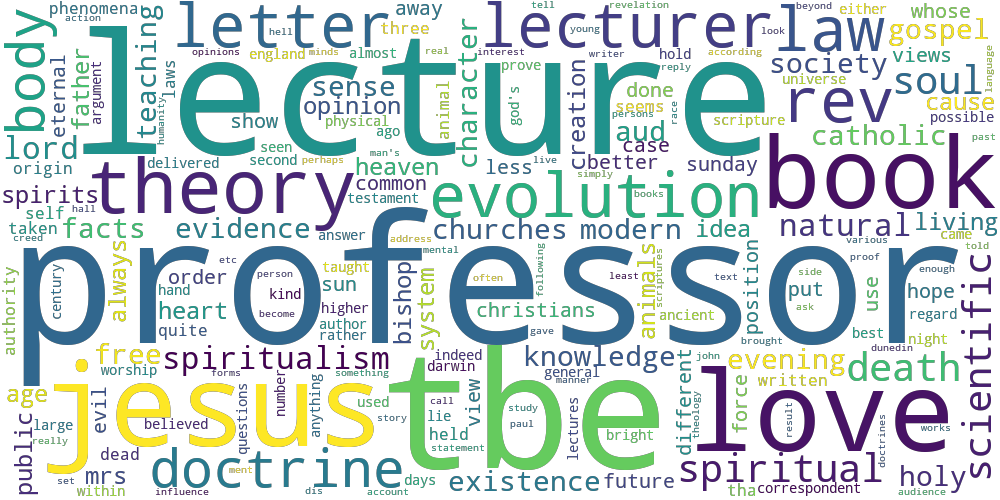
\includegraphics[width=0.9\textwidth]{images/rel_v2_philoso_tf-idf.png}
  \caption{Word cloud for random sample of the Rel corpus.}
  \label{f:wc-rel}
\end{figure}

Having applied the classifier to the NB2 corpora, we generate a word cloud for the resulting Rel corpus (Figure \ref{f:wc-rel}). The indicates some of the main genres of writing we are interested in: public lectures, letters, and perhaps sermons; some of the people that we are interested in: professors, clergy, public lecturers; and some key topics: evolution, creation, and spirituality.

It is argued by \cite{moore} that he `Baconian compromise' between science and religion, according to which the interests of science and religion were distinct, but in harmony with one another, began to lose its hold on many thinkers in the nineteenth century. One reason for this was the development of geological ideas according to which the earth was much older than a certain way of reading of the Bible had suggested, and the introduction of evolutionary theories according to which the various species were not created independently, but evolved from a common ancestor. One manifestation of this was an extreme `conflict' or `warfare' view, according to which science and religion are inherently opposed to one another, while others attempted to find new ways of harmonising the two \cite{dupree}.

\begin{table}[]
        \scriptsize
        \centering
        \begin{tabular}{l|lcr}
        1 & e than the details of mr darwin but this ceaseless & warfare of & the champions of that faith which we at least h \\
        2 & ws during his recent visit to america r review the & warfare of & science by andrew dickson whitb ll d president \\
        3 & re at the pres byterian church last evening on the & warfare of & science and religion there was a moderately goo \\
        4 & in his nbvum organum as quoted by dr white in his & warfare of & science a treatise i commend to the serious att \\
        5 & t between science and keligion nor dr white in his & warfare of & science for one moment assumes tbat there is no \\
      \end{tabular}
      \begin{tabular}{l|lcr}
        6 & l continue to make men wiser and purer dr draper's & conflict of & science and religion is a very interesting book \\
        7 & untested opinions dr drapers con flict is often a & conflict of & science with science of science adopted by reli \\
        8 & ittle as balaam's ass did of hebrew that was not a & conflict of & religion with science but a conflict with nesci \\
        \end{tabular}
        \begin{tabular}{l|lcr}
        9 & ion that there are gratifying signs of decreasing & antagonism between & the church and science while at the same \\
        10 & ant interpretations of the bible rest the fancied & antagonism between & scientific progress and religious truth a \\
        11 & in papers i have not in my lectures presented any & antagonism between &  genesis and geology unless a fair present \\
        12  & perfectly true to say that there is and can be no &  antagonism between &  the church and science whilo at the same  \\
        13  & extending over an indefinite period the apparent &  antagonism between &  science and religion can easily be bridge \\
        14  &  ny dogmatic uit rances now is there any necessary  & antagonism between &  scriptural teaching and the evolution the \\
      \end{tabular}
      \begin{tabular}{l|lcr}
        15  & lecture with a view to reconciling the theory of &  evolution with &  the jewish account of the creation and fall  \\
        16  & idable nature as to the supposed inconsistency of  & evolution with  & the christian belief as to the person of chr \\
        17  & the compatibility or otherwise of the doctrine of  & evolution with &  religious belief professor salmoud as it see \\
        \end{tabular}
        \caption{Selected results from `warfare of', `conflict of', `antagonism between' and `evolution with' concordances.}
        \label{t:rel-concordance}
\end{table}

Both tendencies are present in concordancing results from the Rel corpus (Table \ref{t:rel-concordance}).\footnote{Note that a function was written for the project in order to allow for multi-word concordancing (see `concordance phrase') in the notebook.} Each of the concordance lines seems to address the antagonism or lack of antagonism between religion and science quite clearly. We see this in the case of evolution specifically in lines (1), (15), (16), and (17).\footnote{We also see the closely related issue of the interpretation of biblical book of Genesis in light of geology in (11)} We see discussion in different social contexts, including at churches (3) and public lectures (11). Major international figures are discussed, including Draper and White in(2), (4), (5), (6), and (7). Finally, it is worth noting the name of Salmond, an early New Zealand academic philosophy, who appears in (17) in connection with these issues.



\begin{figure}
    \centering
    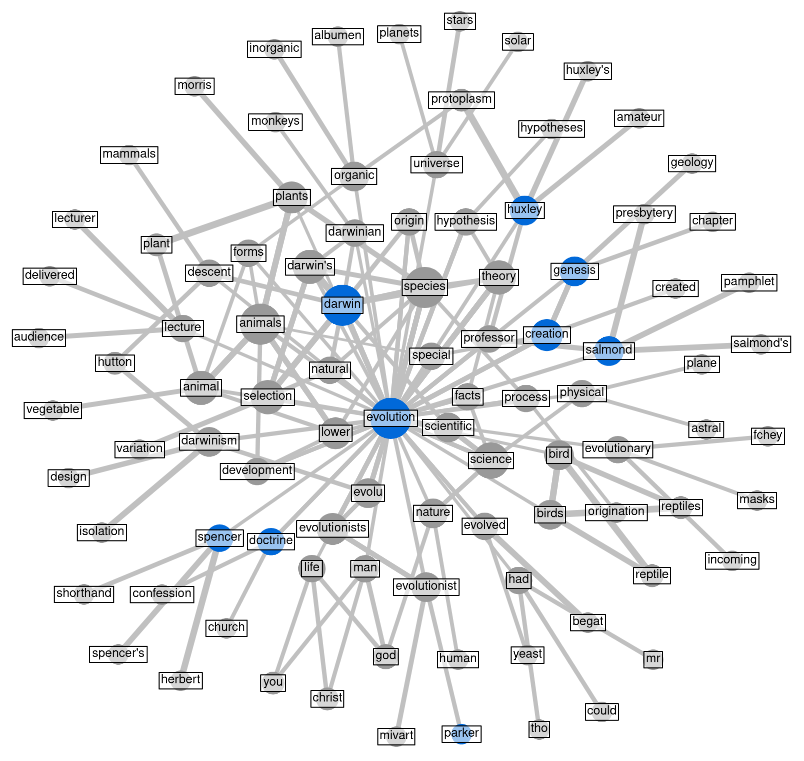
\includegraphics[width=0.7\textwidth]{images/evo_network_main.png}
    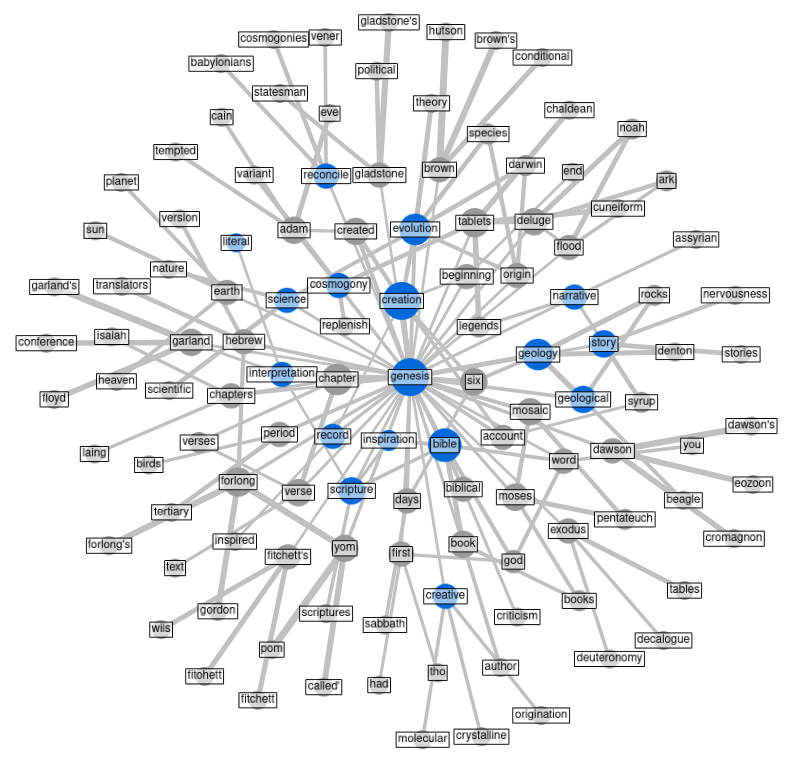
\includegraphics[width=0.7\textwidth]{images/genesis_main.png}
    \caption{\footnotesize{Co-occurrence networks for `evolution' and `genesis' in the Rel corpus, with TF-IDF transformation and log Dice statistic. The top 45 co-occurrences for each are shown along with the four top co-occurrences for each of these. Highlighted nodes are to aid discussion.}}
    \label{f:evo-net}
\end{figure}

Some interesting co-occurrence networks can also be considered.\footnote{The results of collocation analysis are excluded for reasons of space. However, some interesting results are present in `Religion and Evolution in the REL corpus.ipynb'.} Four will be briefly discussed here.\footnote{More such networks can be produced using the project dashboard, linked above or `Religion and Evolution in the REL corpus.ipynb'.}
Figure \ref{f:evo-net} presents co-occurrence networks for `evolution' and `genesis'. One term comes from the side of the sciences and the other from the side of religion. The network for `evolution' indicates the interaction with religious and metaphysical issues of creation and of biblical interpretation insofar as it contains `genesis', `creation', and `doctrine'. We also see some of the names which are associated with evolution in the corpus, including, obviously Darwin, but also his advocate Huxley, the popular philosopher Spencer, who is responsible for the phrase `survival of the fittest' and the local figures Salmond and Parker.\footnote{Parker was a popular public lecturer and academic at Otago, himself mentored by Huxley \cite{crane-2013}.}
The network for `genesis' on the other hand, highlights some of the important questions of biblical interpretation brought on by contact with evolutionary ideas. We again see `evolution' appear, along with `geology', but also various interpretive options including `story', `literal', and `record'. The inclusion of the word `reconcile' again suggests some interest in how religion and the results of the natural sciences might be brought together.

\begin{figure}
    \centering
    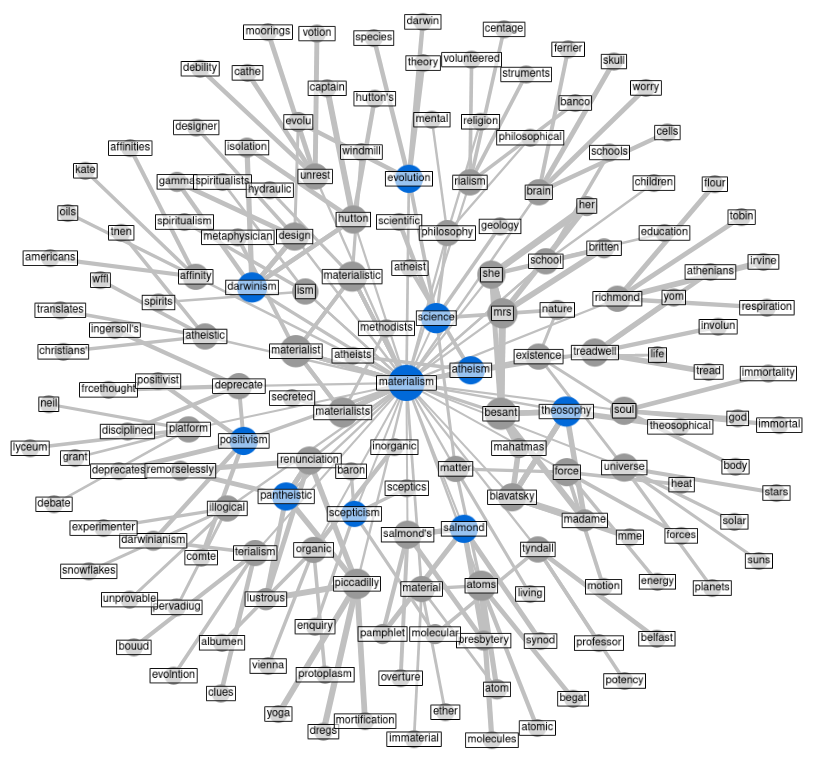
\includegraphics[width=0.7\textwidth]{images/materialism_main.png}
    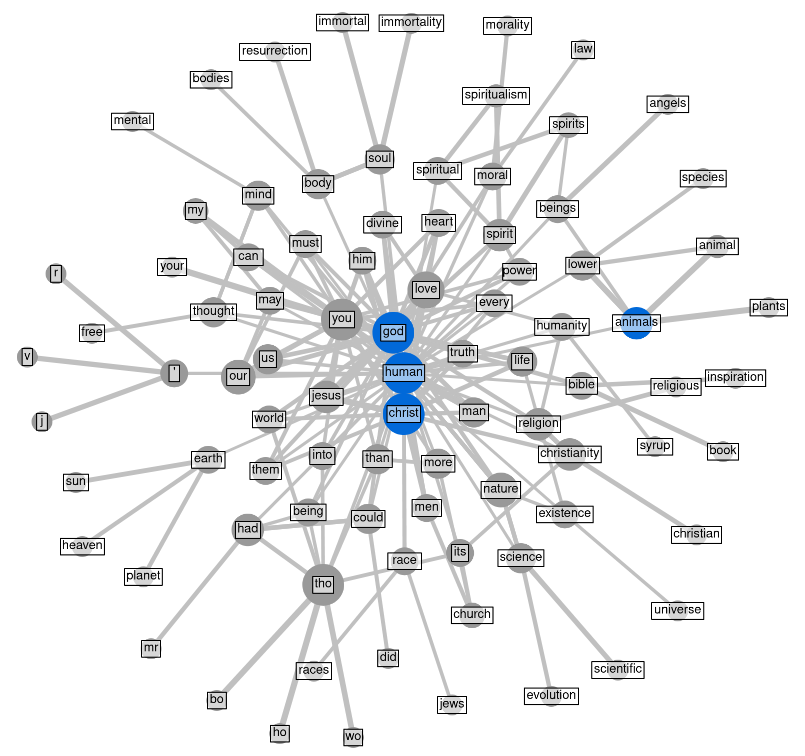
\includegraphics[width=0.7\textwidth]{images/human_net_main.png}
    \caption{\footnotesize{Co-occurrence networks for `materialism' and `human' in the Rel corpus, with TF-IDF transformation and log Dice statistic. The top 45 co-occurrences for `materialism' and the top 50 for `human' are show,  along with the four top co-occurrences for each of these. Highlighted nodes are to aid discussion.}}
    \label{f:human-net}
\end{figure}

Figure \ref{f:human-net} reveals some of the background against which the discussions of evolution and religion were being held. In particular, the network for `human' shows a tight set of interrelationships between spiritual and religious terminology, with the exception of `animal' and `science'. There is less evidence in this network of contestation than in the other networks. The network for `materialism' highlights some of the various alternatives to traditional religious belief that are being discussed in the newspapers at this time and within with evolution would be interpreted. For instance, we see `positivism', `atheism', and `scepticism'. We also see `theosophy', a spiritual movement which was much discussed at the time.\footnote{The term `besant' also appears, for Annie Besant, a travelling theosophical lecturer who toured New Zealand (e.g. \cite{besant}).}


\begin{figure}
    \centering
    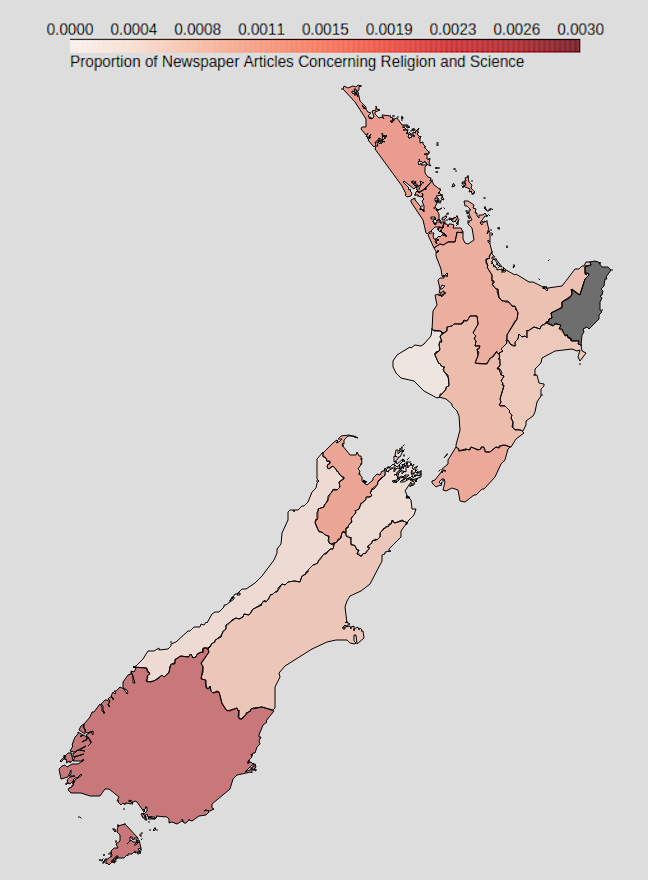
\includegraphics[width=\textwidth]{images/choropleth.png}
    \caption{Choropleth of Rel corpus items as proportion of total items. No newspapers from the Gisbourne region are present in the corpus.}
    \label{f:choropleth}
\end{figure}

The choropleth showing discussion of religion and science by region is presented in Figure \ref{f:choropleth}. They indicate that the majority of this discussion was occurring in Otago. This was is not surprising, as Otago was a major centre for intellectual life in nineteenth century New Zealand. However, drawing strong conclusions from this relies on confidence in the comprehensiveness of both the Rel corpus and the original dataset. This will be discussed later  in the context of problems with labelling (\S \ref{s:discussion}).

\subsubsection{External Validation of the Rel Corpus}\label{s:external-validation}

At this point it is convenient to include a further step of corpus evaluation for the Rel corpus which also applies to the NB1 and NB2 corpora. In the course of this project, a few philosophical pieces on the relationship between religion and science were picked out, but not labelled or otherwise used in the process of corpus construction. In addition, a series of articles about philosophically interesting scientific and religious developments which cite early New Zealand newspaper content were also examined. In order to test the process which led up from the raw Papers Past data to the Rel corpus, we can examine how many of these articles end up being selected by our methods and what has happened to the ones who have not.

Three articles have been used for this step. \cite{ballantyne-2012} offers an account of colonial intellectual life as present in Otago newspapers. In the course of his discussion, he provides a footnote with 15 references to discussions of the value and significance of evolutionary ideas in the Otago newspapers \cite[fn. 53]{ballantyne-2012}. The other two papers are much more specific, dealing with the public lectures of Professor Parker, an Otago academic, protegee of Huxley, and public lecturer on biological topics \cite{crane-2013} and the debates over a pamphlet entitled \emph{The Reign of Grace} by William Salmond, the second philosophy professor employed in New Zealand \cite{wood-2014}. From these articles, ten newspaper mentions of Parker's lectures and six mentions of reports relevant to \textit{The Reign of Grace} are collected. It is expected that the majority of these newspaper articles should be present in the NB2 and Rel corpora.\footnote{Since the Rel corpus is derived by running a classifier on the NB2 corpus, anything in the Rel corpus must also be in the NB2 corpus.}

\begin{table}
  \centering
  \begin{tabular}{l|ll}
    \textbf{Membership} & \textbf{Category} & \textbf{Count} \\
    \hline
    In Rel & & 19 \\
    \hline
    Not in Rel & Composite & 8 \\
     & Too short & 2 \\
     & Parsing error & 2 \\
    & Unexplained & 1 \\
    \hline
    \textbf{Total} & & 32 \\
  \end{tabular}
  \label{t:ext-val}
  \caption{Articles checked for external validation of Rel corpus.}
\end{table}

Table \ref{t:ext-val} summarises the result of checking for the presence of each of these articles, and those which were held out from the labelled data set, in the Rel corpus.\footnote{Additional tables are presented in the Appendix for each source in tables \ref{t:ext-val-chp} to \ref{t:ext-val-crane}.} We see that, the majority are contained in the Rel corpus. This suggests that we are capturing a fairly comprehensive range of the articles about the relationship between philosophy and religion.

Of those articles which are not present in the corpus, the majority are `composite' pieces, either editorials or reports of meetings covering many topics. The shortcomings of the approach to corpus construction have been noted above and will be discussed again in Section \ref{s:discussion}. In terms of the comprehensiveness of the Rel corpus, we should worry that we are missing editorial comment, which might take different positions than those of, say, public lecturers \cite[540--541]{wood-2014}. %check citation again.

Of the remaining missing articles, two are missing as a result of errors in the process of moving from the raw XML files to pandas dataframes. It is not clear what has caused this in the two cases here, but it is not a case of the supervised learning technique failing. Two further missing articles have been removed because they were taken to be too short to be reliably classified. This leaves one article's absence from the corpus unexplained (see Table \ref{t:ext-val-chp}).

\subsubsection{New Zealand Content in the NB2 Corpus}

\begin{table}
  \begin{tabular}{l|l}
    Topic 90 & hipi, toa, tohunga, awa, hymns, pole, ahi, ain't, loafer, like. \\
    Topic 93 & schools, education, children, state, system, religious, bible, school, secular, religion
  \end{tabular}
  \label{t:2-topics}
  \caption{Two topics of interest from 100-topic model of Rel corpus.}
\end{table}

Table \ref{t:2-topics} presents the top ten keywords of the two topics picked out for further investigation.\footnote{The full list of topics and their top-10 keywords for this model is present in `lda\_\-models/rel\_\-v2\_\-philoso\_\-100.csv'.} Topic 90's use of te reo Māori obviously encourages the idea that this topic might have uniquely New Zealand content. However, this would require special expertise not possessed by the investigator.\footnote{
However, note that inspection of documents assigned a high proportion of Topic 90 seemed to reveal a focus on hymns and poetry, without much obvious use ot te reo, although this was not entirely clear. More investigation of this is warranted.
} Discussion of the New Zealand education system has already been noted, leading to interest in Topic 93.

\begin{figure}
  \centering
  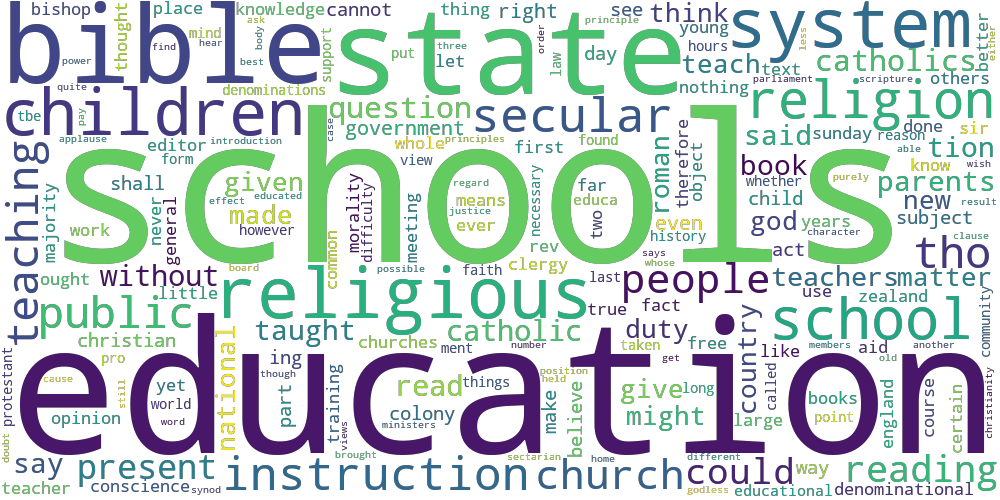
\includegraphics[width=0.9\textwidth]{images/topic93.png}
  \caption{Word cloud for documents with high proportion of Topic 93 in the Rel corpus.}
  \label{f:wc-t93}
\end{figure}

Documents assigned a proportion of Topic 93 above 0.4 were selected for further investigation. A word cloud for these articles is presented by Figure \ref{f:wc-t93}. In addition to the keywords obviously connected to the debate over whether education should be secular or not, we see `zealand' and `colony' indicating some prominence to discussion of these topics in connection with the New Zealand context.

\begin{table}[]
        \scriptsize
        \centering
        \begin{tabular}{l|lcr}
          1 & ons to the following effect were adopted that the  & education act &  should be amended and liberty granted to com \\
          2 & ll of the people if it ba asked why m framing the  & education act &  they did not recognise tbe common religion of \\
          3  & iest nonsense for bishop moran to prate about the  & education act &  being a penal law or to say that it assails t \\
          4  & sixteen years oince by the passing of the present  & education act &  the reading of the bible in schools was forbi \\
          5  & s meeting is further of opinion that tho existing &  education act &  ought to be so amended that sohool committees \\
          6  & r charge whereas the secular character of our own &  education act &  excite deep and widespread dissatisfaction fo \\
          7  & use i the key hrstuaut moved that the exist i ing  & education act &  should be so amended that in i conformity wit \\
          8  & away applau se in asking parliament to around our  & education act &  in the direction of the english act of which \\
          9  & as inconsistent with the secular character of the  & education act &  siv is not this action worthy of eternal repr \\
          10  & o our legislators and ask for an amendment of the  & education act &  in such a direction without first according t \\
      \end{tabular}
      \caption{Selected concordance results for `education act' in documents high in Topic 93.}
      \label{t:nz-concordance}
\end{table}


This New Zealand connection can be confirmed by examining some of the articles high in this topic.\footnote{In the `NZ content.ipynb' notebook, the articles containing the term `zealand' are explored.} The article `ODT\_\-18800630\_\-ARTICLE24' was found to be particularly revelatory of the context of these discussions. It is a letter to the editor in which the passing of the Education Act of 1877, which established secular education for Pākehā \cite{education-act}, is argued against on the basis of features of New Zealand public opinion and that secular education would undermine the quality of the youth of the nation. Further evidence of the prominence of this topic is provided by the selected concordance results in Table \ref{t:nz-concordance}. Of the documents high in Topic 93, around 16\% contain the phrase `education act'.

Here, then, is evidence to answer the third question in the affirmative. We can find evidence of specifically New Zealand-based philosophical issues being discussed in the NB2 corpus. This shows that the corpus has some use for investigation of philosophy and philosophical discourse in colonial New Zealand.

\section{Discussion}\label{s:discussion}

This section reflects on the successes and failures of the project, in turn, and then considers the possibilities for others to use the same methods and workflow for their own projects.

Most importantly, this project shows that a single researcher can quite quickly produce a corpus for the investigation of a particular area of discourse by labelling a small set of articles and using it to train a classifier. This is to answer the first research question with a `yes'. It also revealed some of the ways in which insight into the subject matter can be achieved using data science methods. We found both the presence of a wide range of views on the relationship between religious belief and the sciences, including the involvement of local academics and non-academics. This was sufficient to satisfy the second research question. We also saw how unsupervised methods could be applied on the corpus to find interesting debates concerned with specifically New Zealand-based issues. Methods of this sort could greatly contribute to telling a better and more detailed story about the history of philosophical discourse in New Zealand in the nineteenth century than has previously been accomplished.

Two main shortcomings are worth noting. First, in the discussion of the classifier results, it became clear that the borderline between `philosophy' and `non-philosophy' was somewhat blurry, and that this limited the training of the Naive Bayes classifier. It also seemed that ethics and politics content was being left out more frequently than religious content. This could suggest some bias in the labelling carried out by the investigator.\footnote{However, note the prominence of `God' in the Philoso corpus word cloud (Figure \ref{f:wc-philoso}). This is before any influence of the labelled dataset, and suggests that religious material is just very prominent amongst the intellectual content in early New Zealand newspapers. One way to test for bias would be to perform some additional `external validation' using already existing research on ethical debates in early New Zealand. However, this was not possible given time constraints on the project.}
Moreover, some of the labels initially set up, notably the `metaphysics-epistemology' label, were not used much. Given this, it would be useful to establish a more clear set of criteria for labelling articles.\footnote{Suggestions in this direction are set out in the notebook `Relabelling.ipynb'.}

Another problem which has been discussed above, and is related to the issue of labelling, is the presence of composite articles in which a small proportion is `philosophical'. Many editorials are in this class, and so a whole genre of intellectual activity in early New Zealand newspapers may be being lost from the corpus. A solution to this would be to apply labels at the `text block' level and then to classify an article as philosophy if it contains a block classified as philosophical. This issue is related to the problem of labelling insofar as one of the difficulties confronted in labelling was whether or not to label composite articles as philosophical.

The project was encouraged by the release of the National Library Papers Past Newspaper Open Data Pilot. It seems plausible that there is more material of interest to the historian of philosophy in the National Library's digitised magazines and journals, rather than their newspapers. However, it is important here to remember Ballantyne's point that New Zealand newspapers were `the fundamental infrastructure for intellectual life' in Otago, and that this was helped by the economic impossibility of sustainable periodicals and large collections of imported books \cite[57--58]{ballantyne-2012}. This does encourage the idea that newspapers in New Zealand are an important source of intellectual material in their own right.

Turning to the use of this project by other researchers, the publicly accessible dashboard for the project at \url{nz-newspaper-philosophy.herokuapp.com} enables other researchers to produce co-occurrence networks and explore the NB2 and Rel corpora to attempt to generate some insight about philosophical discourse in early New Zealand newspapers. The corpora produced in the project are also available through links of the dashboard for researchers to explore them using their own tools.

This project also provides general patterns which could easily be followed by other researchers. The basic workflow for labelling and training classifiers is not confined to philosophical discourse. This is also true of the steps to move from ALTO/METS XML files to Pandas dataframes and thus into the Python ecosystem. Given the prevalence of the ALTO/METS standard in newspaper digitisation projects, it is likely that the methods used in this project are quite widely applicable.

\section*{Conclusion}

This report has presented work towards at DATA601 summer project. It was divided into two main tasks: the construction of a useful corpus for investigators in the history of philosophy from the National Library's Papers Past newspaper open data pilot dataset, and the demonstration of some of the uses to which this corpus might be put by digital humanities investigators.

Three research questions were considered, all of which have been answered in the affirmative. First, the project has demonstrated that a useful corpus can be produced using supervised learning techniques with researcher labelling of a small subset of articles and the use of simple Naive Bayes classifiers. Second, it has been shown that insight into the content of discussion about religious belief and the development in the natural sciences, especially evolution, can be obtained from the resulting corpus. %It was also shown that insight into the hotspots of such debates could also be found.
Finally, the discovery, by means of topic modelling and the use of simple word clouds, of the presence and prominence of debates over the nature of education and the way it should be organised in New Zealand in the lead up and wake of the 1877 Education Act, showed that New Zealand focused content is present within the corpus.

It is hoped that process of corpus construction set out in this report can be of use to other researchers with other interests in the dataset. It is also hoped that the corpus produced in part one of this project, and the labelled dataset which enabled the training of classifiers, might be of use to other researchers interested in carrying out digital humanities research on philosophy and intellectual life in general in colonial New Zealand.

\begin{sloppypar}
\printbibliography
\end{sloppypar}

\pagebreak

\renewcommand\thesection{\Alph{section}}
\setcounter{section}{0}
\setcounter{subsection}{0}
\setcounter{table}{0}
\section{Appendix}

This appendix contains tables too large and detailed for the body text.

\begin{table}[h]
  \footnotesize
  \begin{tabular}{l|p{0.3\linewidth}p{0.1\linewidth}p{0.2\linewidth}}
    \textbf{Article} & \textbf{Title} & \textbf{Philosophy Type} & \textbf{Description}\\
    \hline
    AS\_\-18760720\_\-ARTICLE20 &	GRANDMAMA ON "WOMAN'S RIGHTS."  &	Ethics &	Correctly labelled \\
    AS\_\-18820306\_\-ARTICLE31 &	THE BRADLAUGH EPISODE. &	Ethics & Correctly labelled \\
    AS\_\-18881121\_\-ARTICLE77 &	"PROGRESS and AFTERWARDS." &	Ethics &	Correctly labelled \\
    DSC\_\-18600731\_\-ARTICLE28 &	Friday, July 13.	 & Other & Correctly labelled  \\
    DSC\_\-18601225\_\-ARTICLE10 &	LETTERS In Reply to Sir William Martin's Pamphlet on the Taranaki Question.  No. 1. & Ethics & Correctly labelled	\\
    DTN\_\-18940820\_\-ARTICLE7 &	The Daily Telegraph. MONDAY, AUGUST 20,1894. THE ROLLESTON BANQUET. & Ethics &	Mislabelled (passing reference) \\
    ESD\_\-18890826\_\-ARTICLE1 &	COLONIALCHARACTERISTICS	 & Ethics &	Mislabelled \\
    LT\_\-18831025\_\-ARTICLE34 &	TIMARU TALK. & Other &	Composite \\
    LT\_\-18970507\_\-ARTICLE14 &	CAPITAL PUNISHMENT.	 & Ethics &	Correctly labelled \\
    LT\_\-18980920\_\-ARTICLE26 &	CURRENT TOPICS. &	Ethics &	Composite \\
    NEM\_\-18800301\_\-ARTICLE9 &	The Nelson Evening Mail.  MONDAY, MARCH 1, 1880.  NIHILISM : WHAT IS IT ? &	Ethics &	Correctly labelled. \\
    NZTIM\_\-18780509\_\-ARTICLE5 &	UNTITLED & Ethics &	Composite \\
    ODT\_\-18830714\_\-ARTICLE20 &	PASSING NOTES.	& Ethics &	Composite \\
    OO\_\-18970911\_\-ARTICLE4 &	BLACKMAILING. &	Ethics &	Correctly labelled \\
    WI\_\-18470303\_\-ARTICLE5 &	ORIGINAL CORRESPONDENCE. &	Ethics & Mislabelled (passing reference) \\ %Argues that some philosophical discussion about the purpose of education ought to happen, but doesn't actually offer any.
  \end{tabular}
  \caption{Full list of false negatives from test set for second Naive Bayes classifier.}
  \label{t:false-negatives-full}
\end{table}



\begin{table}
  \footnotesize
  \begin{tabular}{l|p{0.3\linewidth}p{0.1\linewidth}p{0.2\linewidth}}
    \textbf{Article} & \textbf{Title} & \textbf{Readable} & \textbf{Description}\\
    \hline
    AG\_\-18990504\_\-ARTICLE7	&	Ashburton Guardian. Megna est Veritas et Prævalebit. THURSDAY, MAY 4, 1899.	&	True	&	Correctly labelled (quack advertisement)	\\
    CHP\_\-18951209\_\-ARTICLE55	&	ST. ALBANS WESLEYAN CHURCH.	&	True	&	Composite (religious)	\\
    ESD\_\-18851028\_\-ARTICLE1	&	WHITE CROSS SOCIETY.	&	True	&	Edge case (religious)	\\
    ESD\_\-18891218\_\-ARTICLE59	&	CHARACTERISTICS OF CHIRISTIANITY.	&	True	&	Mislabelled (religious)	\\
    ESD\_\-18960111\_\-ARTICLE47	&	MB RELIGIOUS WORLD 'HUMAN ONENESS.'	&	True	&	Mislabelled (religious)	\\
    GRA\_\-18960522\_\-ARTICLE19	&	THE NEW PHOTOGRAPHIC PROCESS,	&	True	&	Correctly labelled (materials of warships)	\\
    LT\_\-18801016\_\-ARTICLE32	&	CANTERBURY COLLEGE.	&	True	&	Correctly labelled (list of graduations)	\\
    LWM\_\-18950614\_\-ARTICLE27	&	Select Poetry.	&	True	&	Correctly labelled (religious)	\\
    ME\_\-18870708\_\-ARTICLE32	&	THE MYSTERY OF INSTINCT.	&	FALSE	&	A few philosophical terms are readable.	\\
    NEM\_\-18920606\_\-ARTICLE29	&	THE POPE ON ITS DIFFICULTIES.	&	True	&	Edge case (religious)	\\
    ODT\_\-18850204\_\-ARTICLE30	&	THE CATHOLIC CLAIMS T. BIBLEREADING IN SCHOOLS.	&	True	&	Correctly labelled (religious)	\\
    ODT\_\-18980407\_\-ARTICLE89	&	THE INFLUENCE OF CHRISTIANITY. TO THE EDITOR.	&	True	&	Correctly labelled (religious)	\\
    ODT\_\-18981013\_\-ARTICLE51	&	DEAN FARRAR DEFENDS THEATRE-GOING.	&	True	&	Correctly labelled (religious)	\\
    OW\_\-18770317\_\-ARTICLE59	&	BISMARCK.	&	True	&	Mislabelled (religious)	\\

  \end{tabular}
  \caption{Full list of false positives from test set for second Naive Bayes classifier.}
  \label{t:false-positives-full}
\end{table}


\begin{table}
  \footnotesize
  \begin{tabular}{l|lllll}
    \textbf{Article} & \textbf{philoso*} & \textbf{NB 1} & \textbf{NB 2} & \textbf{Rel} \\
    \hline
    %CHP\_\-18940707\_\-ARTICLE3 & True & True & True & True \\ in labelled
    CHP\_\-18921024\_\-ARTICLE53 & False & True & True & True & \\
    CHP\_\-18991023\_\-ARTICLE39 & False & True & True & True & \\
    CHP\_\-18630117\_\-ARTICLE3 & True & False & False & False & Unexplained\\
    %CHP\_\-18930322\_\-ARTICLE47 & False & True & True & True \\ in labelled
    %CHP\_\-18950607\_\-ARTICLE45 & False & True & False & False & \\ Music - issue for nb2
    WI\_\-18710720\_\-ARTICLE13 & True & True & True & True & \\
  \end{tabular}
  \caption{Articles identified but not in labelled collection.}
  \label{t:ext-val-chp}
\end{table}

\begin{table}
  \footnotesize
  \begin{tabular}{l|lllll}
    \textbf{Article} & \textbf{philoso*} & \textbf{NB 1} & \textbf{NB 2} & \textbf{Rel} & \textbf{Note}\\
    \hline
    ODT\_\-18710509\_\-ARTICLE18 & False & True & True & True & Used in training \\
    TT\_\-18710720\_\-ARTICLE23 & False & False & False & False & XML parse error \\
    OW\_\-18730531\_\-ARTICLE11 & False & True & True & True & \\
    ODT\_\-18760516\_\-ARTICLE22 & False & True & True & True & \\
    OW\_\-18760520\_\-ARTICLE81 & False & True & True & True & \\
    OW\_\-18760527\_\-ARTICLE71 & False & True & True & True & \\
    ODT\_\-18760617\_\-ARTICLE20 & False & True & True & True & \\
    OW\_\-18780907\_\-ARTICLE28 & False & True & True & True & \\
    ST\_\-18800924\_\-ARTICLE14 & False & False & False & False & XML parse error\\
    ODT\_\-18801204\_\-ARTICLE15 & False & True & True & True & \\
    OW\_\-18820701\_\-ARTICLE45 & False & True & True & True & \\
    OW\_\-18820701\_\-ARTICLE77 & False & True & True & True & \\
    ODT\_\-18820705\_\-ARTICLE26 & False & True & True & True & \\
    OW\_\-18820708\_\-ARTICLE61 & False & True & True & True & \\
    ME\_\-18940605\_\-ARTICLE7 & False & False & False & False & Filtered (too short) \\
  \end{tabular}
  \caption{Articles on evolutionary ideas identified in Ballantyne 2012.}
  \label{t:ext-val-bal}
\end{table}

\begin{table}
  \footnotesize
  \begin{tabular}{l|lllll}
    \textbf{Article} & \textbf{philoso*} & \textbf{NB 1} & \textbf{NB 2} & \textbf{Rel} & \textbf{Note} \\
    \hline
    ODT\_\-18880705\_\-ARTICLE21 & False & True & True & True & \\
    ODT\_\-18880906\_\-ARTICLE30 & False & True & False & False & Composite (synod report)\\
    ODT\_\-18881101\_\-ARTICLE18 & False & True & False & False & Composite (synod report)\\
    ODT\_\-18881102\_\-ARTICLE31 & False & True & False & False & Composite (synod report)\\
    ODT\_\-18881103\_\-ARTICLE24 & False & True & False & False & Composite (synod report)\\
    ODT\_\-18881108\_\-ARTICLE3 & False & False & False & False & Filtered (too short)\\
  \end{tabular}
  \caption{Articles on 'Reign of Grace' controversy identified in Wood 2014.}
  \label{t:ext-val-wood}
\end{table}

\begin{table}
  \footnotesize
  \begin{tabular}{l|lllll}
    \textbf{Article} & \textbf{philoso*} & \textbf{NB 1} & \textbf{NB 2} & \textbf{Rel} & \textbf{Note}\\
    \hline
    ODT\_\-18810528\_\-ARTICLE13 & True & True & True & True & \\
    OW\_\-18810604\_\-ARTICLE108 & False & False & False & False & Filtered (too short)\\
    OW\_\-18820701\_\-ARTICLE77 & False & True & True & True & \\
    NOT\_\-18840128\_\-ARTICLE15 & False & True & True & True & \\
    ODT\_\-18840923\_\-ARTICLE8 & False & False & False & False & Composite\\
    ODT\_\-18850602\_\-ARTICLE17 & False & True & True & True & \\
    ODT\_\-18950927\_\-ARTICLE6 & False & False & False & False & Composite\\
    ODT\_\-18910723\_\-ARTICLE10 & False & False & False & False & Composite\\
    ODT\_\-18820629\_\-?? & N/A & N/A & N/A & N/A & Advertisement\\
    ODT\_\-18861120\_\-ARTICLE3 & False & False & False & False & Composite\\
  \end{tabular}
  \caption{Material concerning Fletcher's public lectures on evolution identified in Crane 2013.}
  \label{t:ext-val-crane}
\end{table}



\end{document}
